\documentclass[11pt,a4paper,twoside]{article}
\usepackage[utf8]{inputenc}
\usepackage{amsmath}
\usepackage{amsfonts}
\usepackage{amssymb}
\usepackage{graphicx}
\usepackage{physics}
\usepackage{mathtools}
\usepackage{bm}
\usepackage{bbm}
\usepackage{booktabs}
\author{François Coppens}
\title{Notes}
\renewcommand{\vec}[1]{\bm{\mathrm{#1}}}
\newcommand{\unit}[1]{\,\mathrm{#1}}
\newcommand{\diff}[1]{\,\mathrm{d}{#1}}
\begin{document}

	Superfluids are liquids and gasses with remarkable properties. In particular, superfluid helium can flow through a capillary without friction[\emph{ref}] due to its extremely low viscosity[https://doi.org/10.1016/j.crhy.2017.10.016]($\approx\!1500$ times lower than normal liquid helium), or creep up the wallof a container, seemingly defying the force of gravity (``Rollin creeping'')[\emph{ref}]. Its thermal conductivity is about $3\times10^6$ times higher[\emph{ref}] than that of typical liquids and about 200 times higher[\emph{ref}] than that of copper at room temperature[https://doi.org/10.1016/S0031-8914(36)80312-7,https://doi.org/10.1038/140062a0]. It therefore earned the title of ``best heat conducting substance we know'' by Willian and his daughter Anna Keesom and dubbed `\emph{supra-heat-conducting}'[\emph{ref}]. Later it was understood why[\emph{ref}] and it turns out that heat doesn't diffuse through the medium as in normal liquids, but rather it travels through the medium in waves (second sound). This makes it an ideal coolant e.g. to stabilise the superconducting magnets in CERN's Large Hadron Collider[ref]. Helium is also the only known substance that stays liquid at zero temperature and low pressures and both it's angular momentum and vorticity are quantised, making it the first observed macroscopic quantum substance. Helium-4 becomes superfluid below the$\lambda$-point, named so by William H. Keesom in 1936 who measured a singularity in the specific heat at $T_\lambda=2.2\unit{K}$.[https://doi.org/10.1016/j.crhy.2017.10.016]\\
	
	\begin{figure}[t]
		\begin{center}
			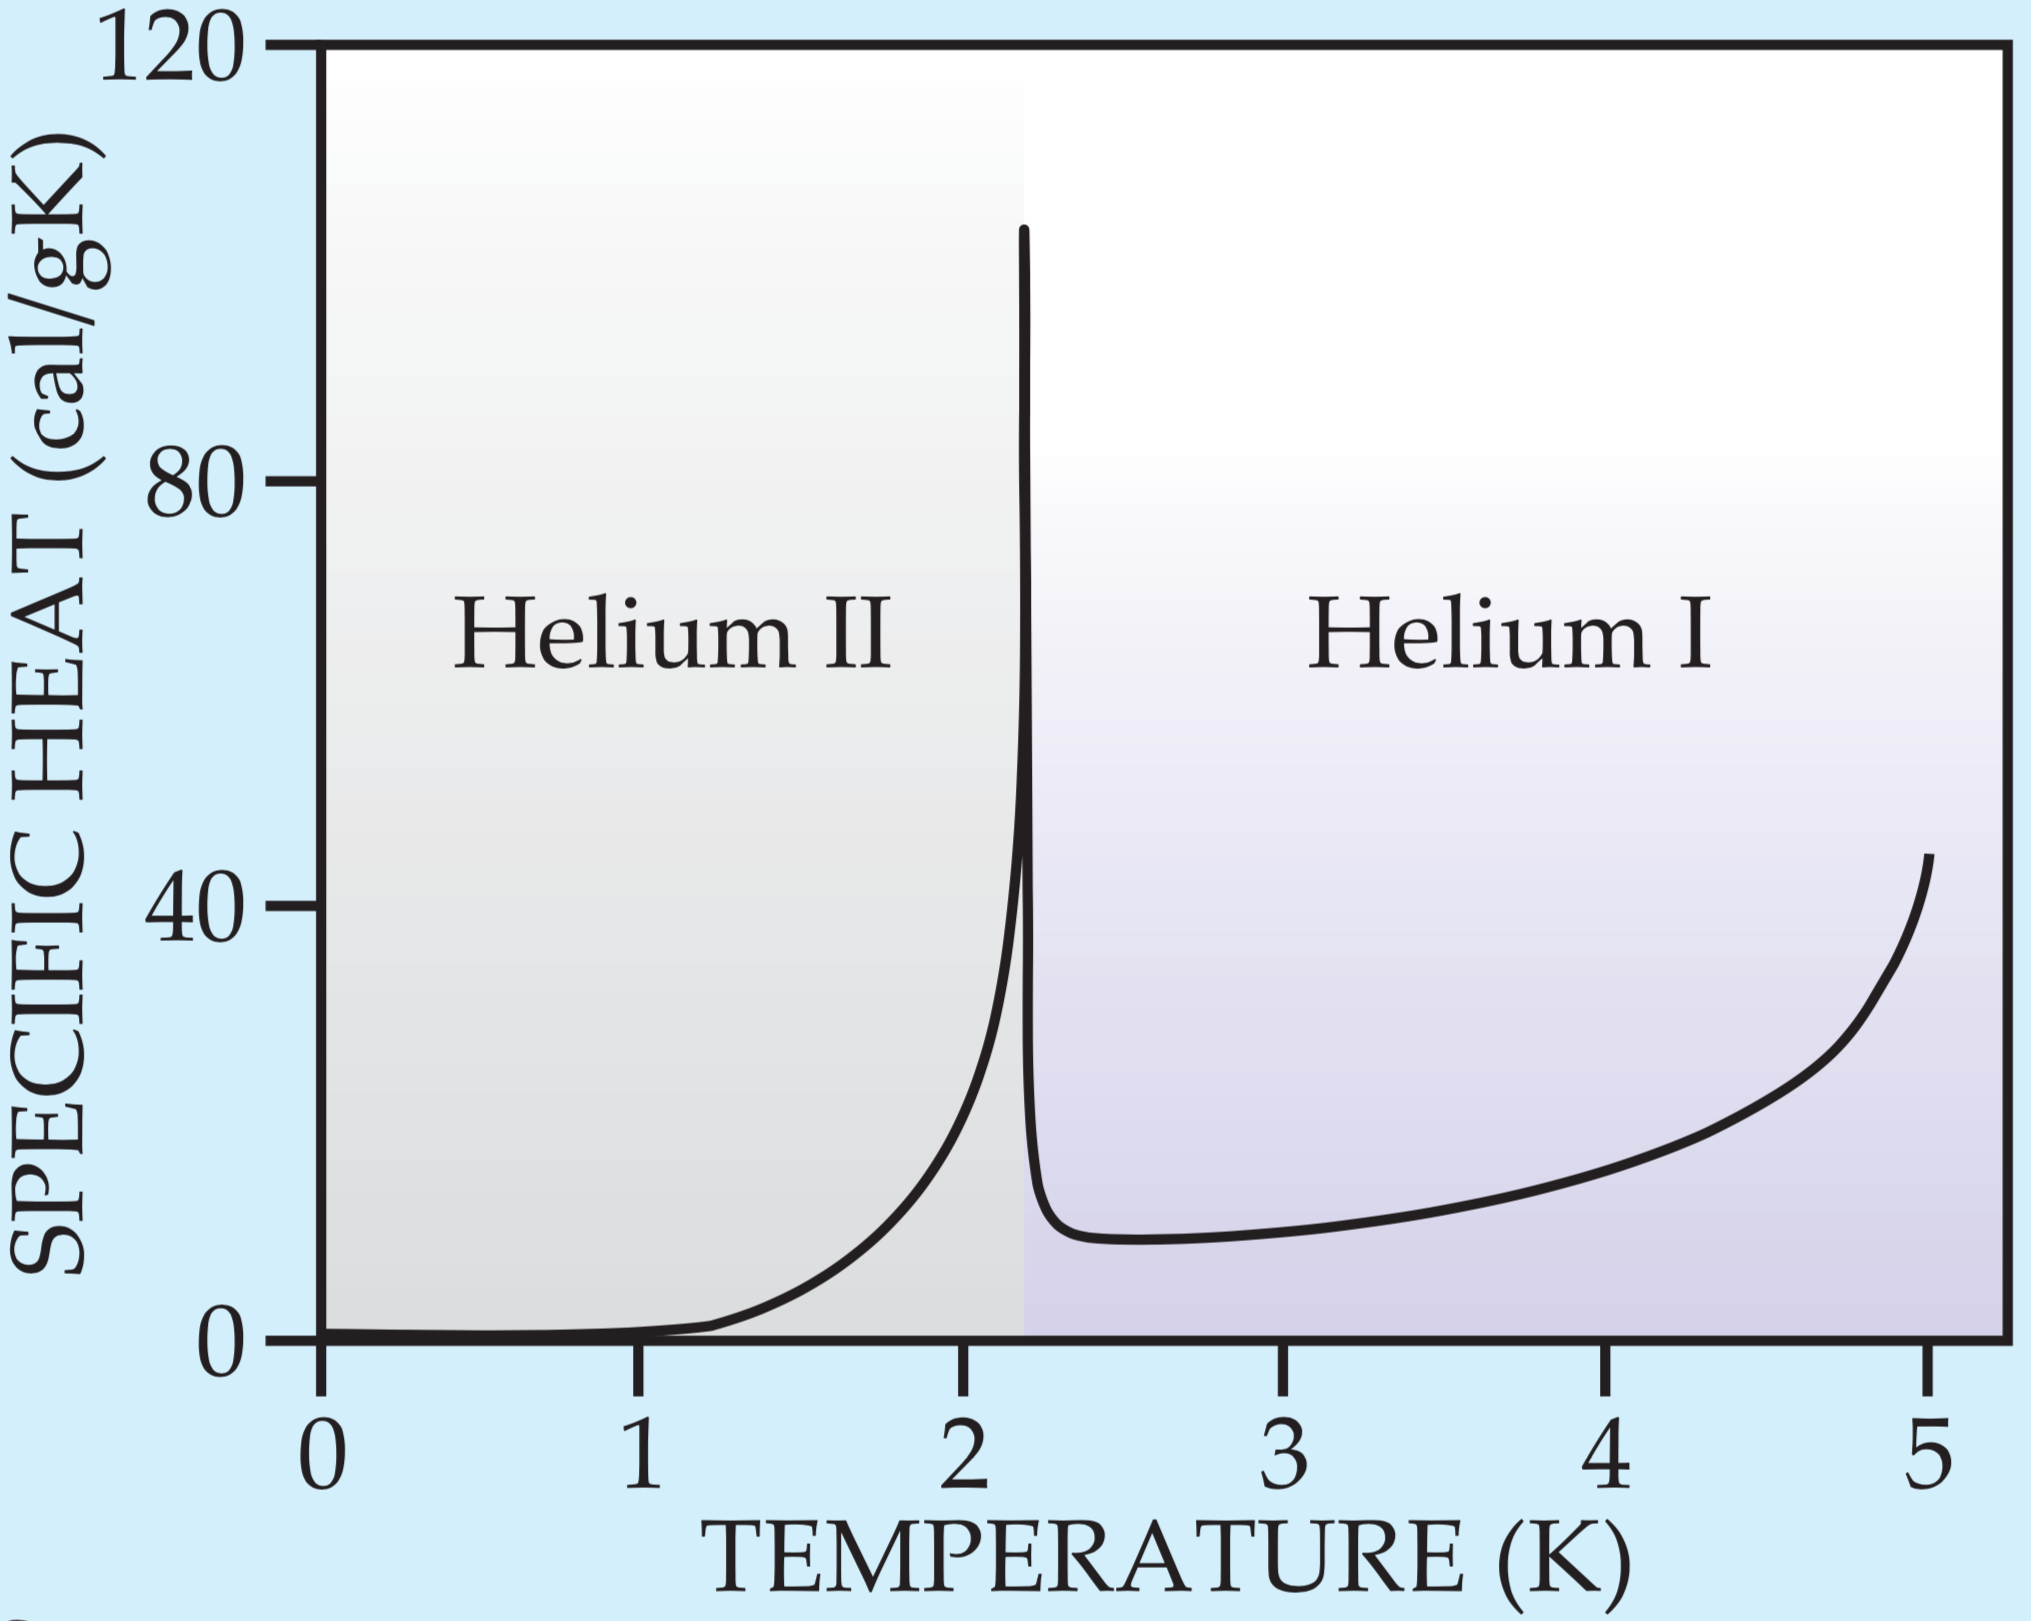
\includegraphics[width=0.75\textwidth]{specific-heat}
		\end{center}
		\caption{The specific heat of $^4$He as a function of the temperature. There is a clearly visible singularity around $2.2\unit{K}$ and the graph itself has the distinct $\lambda$-like shape that inspired Willem and Anna Keesom to call the temperature at which the singularity occurs the ``$\lambda$-point''.}
		\label{fig:specific-heat}
	\end{figure}	
	
	\section{A brief history of superfluidity}
		Helium was the last gas to be liquefied and was done so by Kamerlingh Onnes in 1908[\emph{ref}]. In 1932 John McLennan saw[\emph{ref}] that liquid helium stopped boiling below $\approx\!2.2\unit{K}$ and later that year Willem Keesom and his daughter Anna observed[\emph{ref}], while measuring  the temperature dependence of the specific heat, a singularity around the same temperature. They called it the ``$\lambda$-temperature'',  $T_\lambda$, because of the shape of the temperature dependence of the specific heat resembling the Greek letter $\lambda$ (see Figure \ref{fig:specific-heat}). A few years later in 1935 Burton measured a sharp decrease in the viscosity of liquid helium below $T_\lambda$. Around the same time Fritz London was already thinking about macroscopic wave functions and why helium does not freeze at $T=0\unit{K}$ under atmospheric pressure. He concluded that it was caused by the zero point motion of the helium atoms and of their associated kinetic energy that was comparable to their Van der Waals energy, effectively preventing liquid helium to solidify. The year after, in 1936, Willem and Anna Keesom measured an abnormally high heat conductance below $T_\lambda$. This was confirmed roughly one year later by J.F. Allen \emph{et al.} and it was understood that the high thermal conductance was the reason for the helium to stop boiling whenever the temperature drops below $T_\lambda$. It was in 1937 when Kapitza tried to determine the viscosity of the laminar flow that he measured a viscosity that was about $10^4$ times smaller than that of hydrogen gas. It was then that Kaptiza who, by analogy with superconductors, first coined the word ``superfluid'' to describe the special state that helium enters below the $\lambda$-point where it can flow, seemingly without friction. Allen and Misner realised that superfluid helium is not just a liquid with a very low viscosity, but that its hydrodynamics was completely different from that of ordinary liquids and therefore required a completely new interpretation.\\
		
		The start of this new interpretation was made by London in 1938 when he made a connection between the behaviour of superfluid helium to that of an ideal Bose-Einstein gas. Both his calculated value for $T_c=3.09\unit{K}$ and the behaviour of the temperature dependence of the heat capacity for the ideal Bose-gas were very similar to the measured ones for liquid helium below $T_\lambda$. He wrote to Nature that ``it was difficult not to imagine a connection with Bose-Einstein condensation''. Laszlo Tisza expanded upon London's ideas and considered a Helium II system of total $N$ atoms to consist of two parts; a macroscopic ``condensed'' part $n_0$, the superfluid component, in the ground state, and the remaining part $n=N-n_0$, the normal component, where the helium atoms are distributed over the excited states. Assuming this was correct the fraction $n_0/N$ should decrease with temperature according to the equation\\

		\begin{align}
			\frac{n}{N} = \qty(\frac{T}{T_0})^s \quad \text{for} \quad T<T_0
		\end{align}

		where $s=3/2$ for an ideal gas and should be taken larger, e.g. $s=5$, for a real liquid with stronger interactions between the atoms.\\
		
		This was the birth of the ``two-fluid'' model. With this model he derived two hydrodynamic equations for liquid helium below $T_\lambda$ and discovered that within it, heat propagates in waves, contrary to diffusing, and calculated their velocity. He also explained why the viscosity is disappearing at low temperatures [\emph{this is explained in the french paper I still have to read}] contrary to classical liquids where the viscosity increases. In 1941 Lev Landau reformulated Tisza's theory on a more rigorous footing. He assumed, contrary to Tisza, that the normal component of the liquid was made-up of collective excitations instead of excited single atoms. He postulated that the liquid could exhibit two states of motion which he called ``potential motion''and ``vortex motion'' corresponding to the cases $\curl{\vec{v}}=0$ and $\curl{\vec{v}} \neq 0$ respectively, and that the corresponding energies are discontinuously separated by an energy gap $\Delta$. In case of potential internal motion  the excitations are quanta of longitudinal (sounds) waves, i.e., phonons. The excitations of the vortex-spectrum could be called ``rotons''(see Figure \ref{fig:phonon-roton}).\\

		\begin{figure}[t]
			\begin{center}
				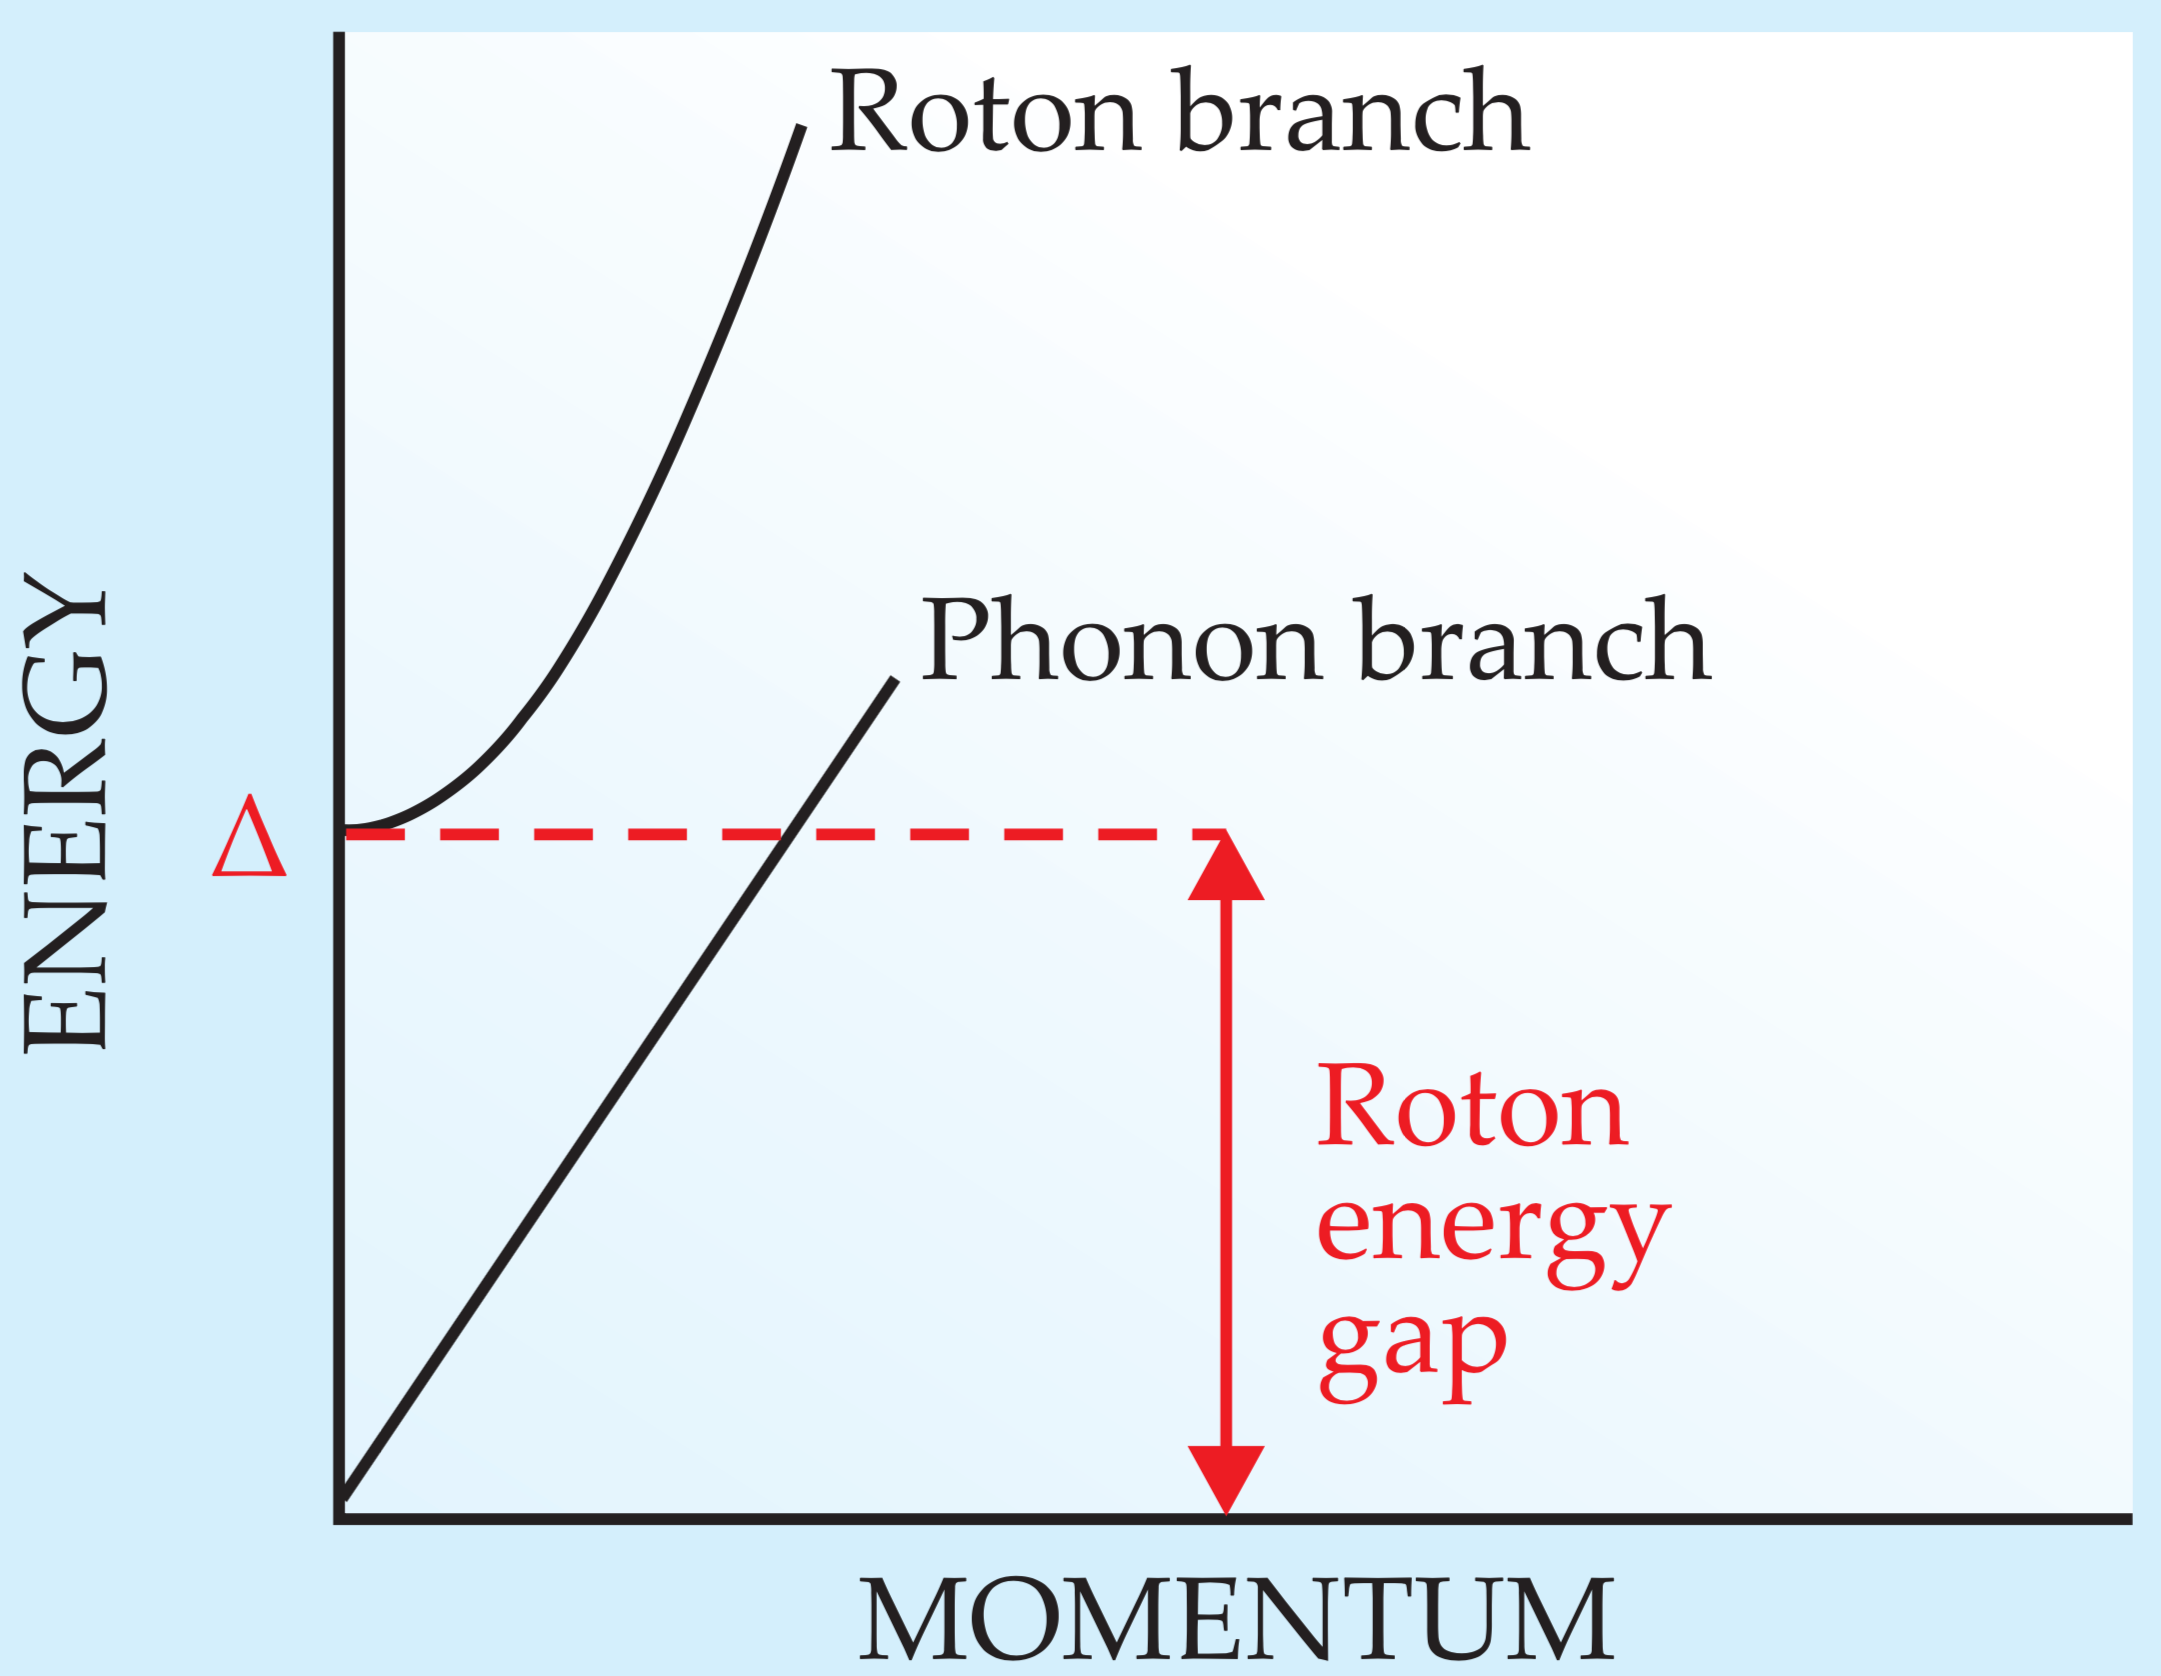
\includegraphics[width=0.495\textwidth]{phonon-roton-landau-first}
				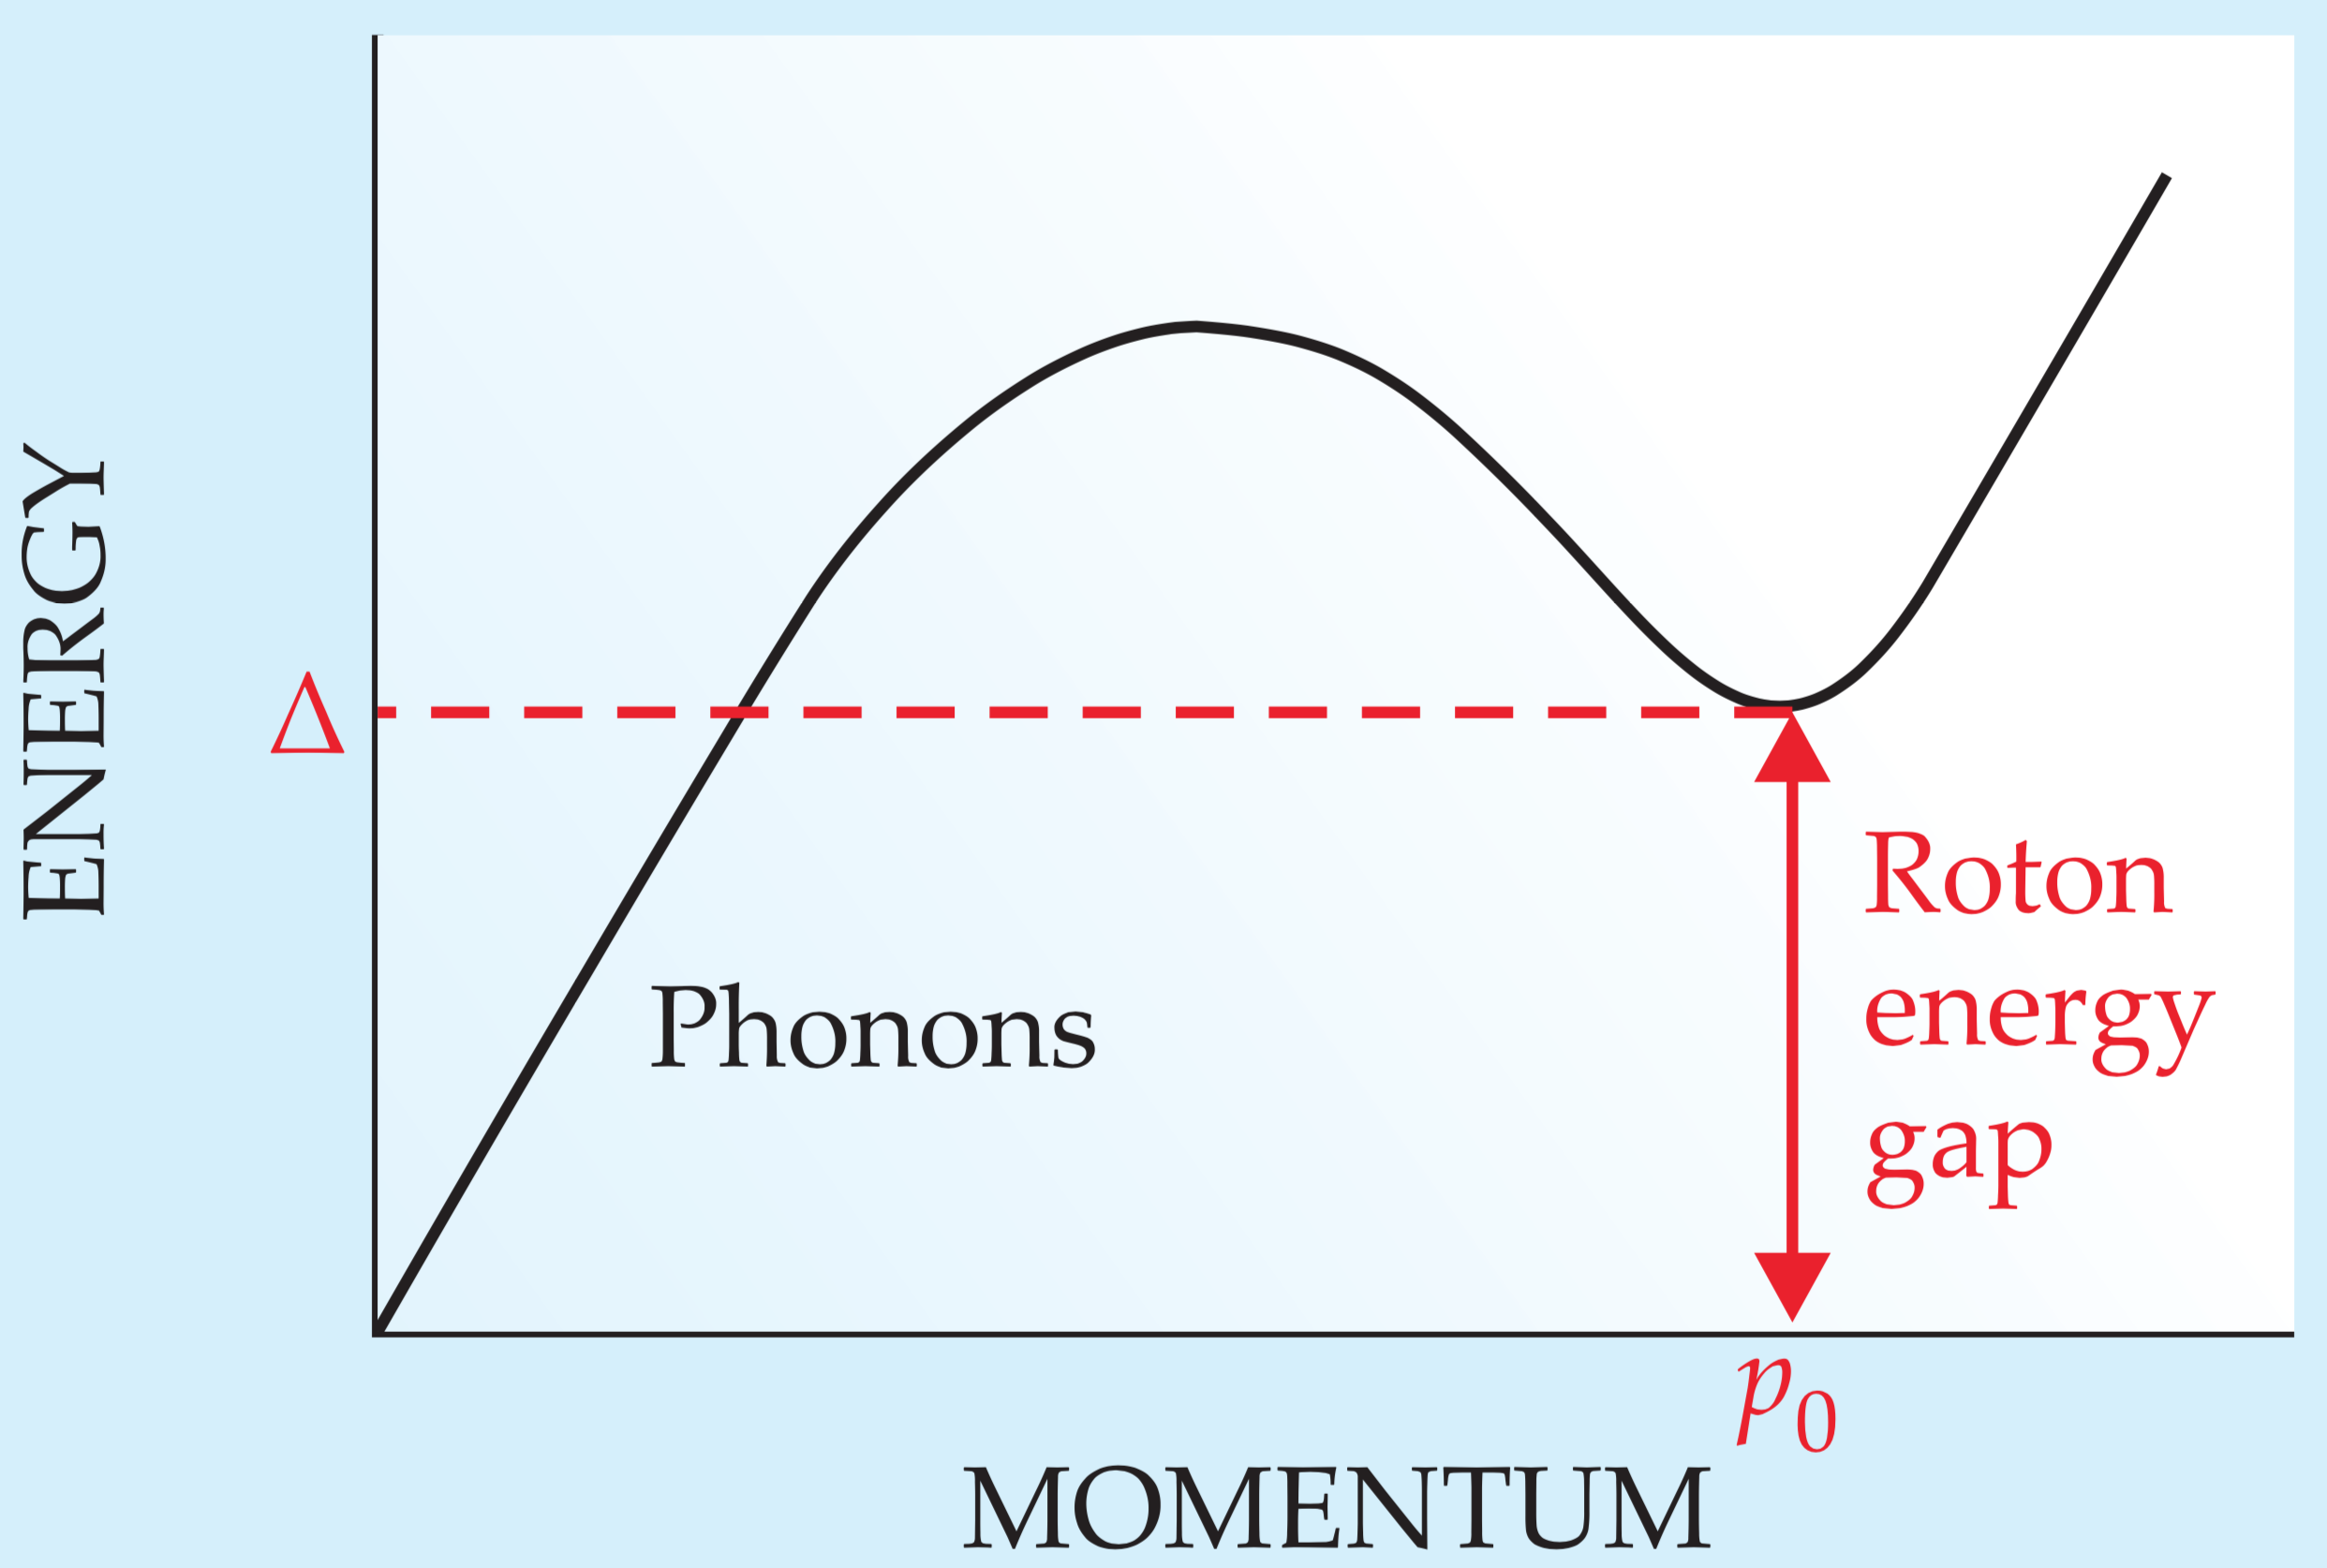
\includegraphics[width=0.495\textwidth]{phonon-roton-bogoliubov}
			\end{center}
			\caption{Left: Lev Landau's 1941 energy dispersion curve for the excitations in liquid helium below $T_\lambda$. It exhibits a phonon- and a roton branch. The slope of the linear phonon branch corresponds to the velocity of sound. Right: Lev Landau's (Bogoliubov's) 1947 corrected dispersion curve. The roton-branch is no longer a separate excitation branch but rather an extension of the phonon-branch.}
			\label{fig:phonon-roton}
		\end{figure}

		A theoretical demonstration, explicitly showing that phonons and rotons are collective excitations of the liquid, came in the form of a 1947 paper by Nikolay Bogolyubov[ref]. The intimate relationship between superfluidity and Bose-Einstein condensation was not universally accepted until 1995 when Cornell and Wienman in Colorado and Ketterle at MIT discovered BEC in rubidium quantum gases[ref].

	\newpage
	\section{Helium droplets}
		Until the 1980, most experimental and theoretical work was done on bulk systems, i.e. systems of the order of $N_A$ number of atoms. It was only in the last couple of decades that advancements in technology enabled experimentalists to create nanoscale sized superfluid helium droplets. From the early 1990's onwards, superfluid helium nano-droplets became an active field of study, both experimentally and theoretically. Surely, the finite size of these droplets would impose some interesting properties as compared to bulk liquid helium.\\
		
		The helium-helium interaction is already weak in bulk liquid helium and in finite self-bound systems such as droplets it is even weaker, e.g. the binding energy per atom is $<\!7.17\unit{K}$. Because of this, helium droplets cool down very rapidly, reaching their limiting temperature of about $0.38\unit{K}$ in microseconds. Pure helium droplets are neutral systems and its properties like their size, binding energy and excitation spectra, are not easy to determine experimentally and are usually obtained by indirect methods. This didn't stop the theoreticians describe doped $^4$He$_N$ droplets using a wide variety of approaches depending on the size and character of the droplets ranging from Quantum Monte Carlo, Hypernetted-Chain/Euler-Lagrange, Variational Monte Carlo and many others.\\
	
		A key property of helium droplets is their ability to pickup any kind of dopants with which they collide, binding them, depending on the relative strength of the He-dopant interaction compared to the He-He interaction, either to their surface (e.g. the alkalies) or absorb them into their interior. They can therefore be doped with almost any kind of atomic or molecular species where they can form new complexes. This enables a broad spectrum of possible experimental study. Due to the fact that helium droplet are ultra cold superfluid liquids, and therefore provide high mobility of any picked-up dopants, one can do high resolution spectroscopy studies. Having a fine control over the number of picked-up dopants[29] one can use droplets as a matrix for creating self-organising structures of polar molecules, or very cold metal clusters and study their Coulomb explosion. From the perspective of the droplet it's possible to use the dopants as gentle probes to determine the superfluid properties of helium droplets that would be inaccessible with other methods. For two examples of this see [37-39], where a dopant is used to probe the superfluid character of small $^4$He droplets and [16,17] to see their limiting temperatures.\\
		
		\begin{figure}[t]
			\begin{center}
				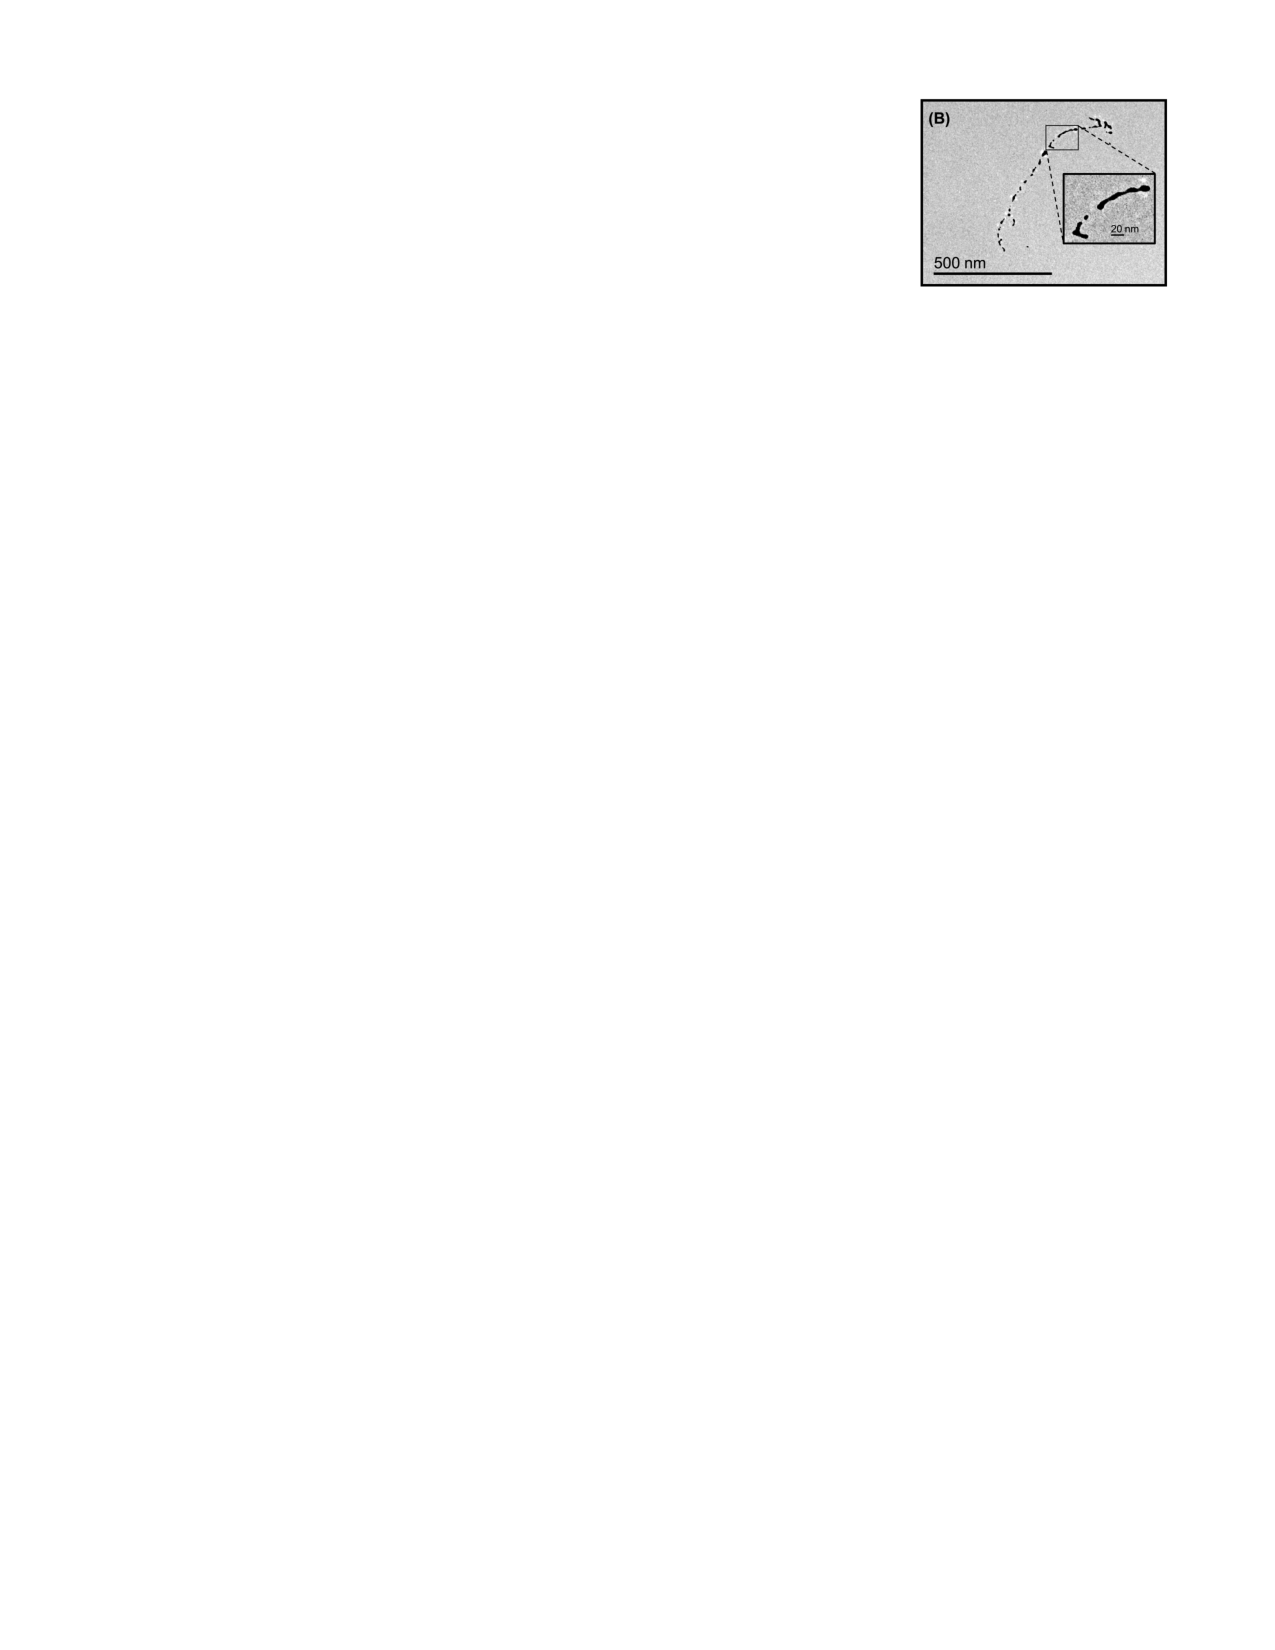
\includegraphics[width=0.75\textwidth]{silver-filament}
			\end{center}
			\caption{Electron-microscope image of and elongated track-shaped Ag-cluster after it is surface-deposited.}
			\label{fig:silver-filament}
		\end{figure}	
				
		One of the most intriguing properties of superfluid helium droplets is the fact that they can host vortices. Because of their ultra low temperature they are true quantum liquids and thus their vorticity and angular momentum are quantised. The existence of quantised vortices was anticipated because they have been created and observed in Bose-Einstein condensates made of dilute gases. However. the detection of quantised vortices is still experimentally challenging. Recently, Gomez, Loginov and Vilesov performed experiments[PRL 108, 155302 (2012)] where vortices inside superfluid $^4$He droplets, produced by the expansion of liquid helium, were traced by introducing Ag atoms which clustered along the vortex lines, into the droplets. The Ag clusters were subsequently surface-deposited and imaged via electron microscopy. The prevalence of elongated track-shaped deposits (see Figure \ref{fig:vortex-array}) shows that vortices are present in droplets larger than about $300\unit{nm}$ and that their lifetime exceeds a few milliseconds. Two years later Gomez reported[Science 345, 906 (2014)] on the formation of quantum vortex lattices inside droplets. He used single-shot femtosecond x-ray coherent diffractive imaging to investigate the rotation of single, isolated superfluid helium-4 droplets containing $\sim\!10^8$ to $10^{11}$ atoms. The formation of quantum vortex lattices inside the droplets was confirmed by observing the characteristic Bragg patterns from xenon clusters trapped in the vortex cores (see Figure \ref{fig:vortex-array}).\\

		\begin{figure}[t]
			\begin{center}
				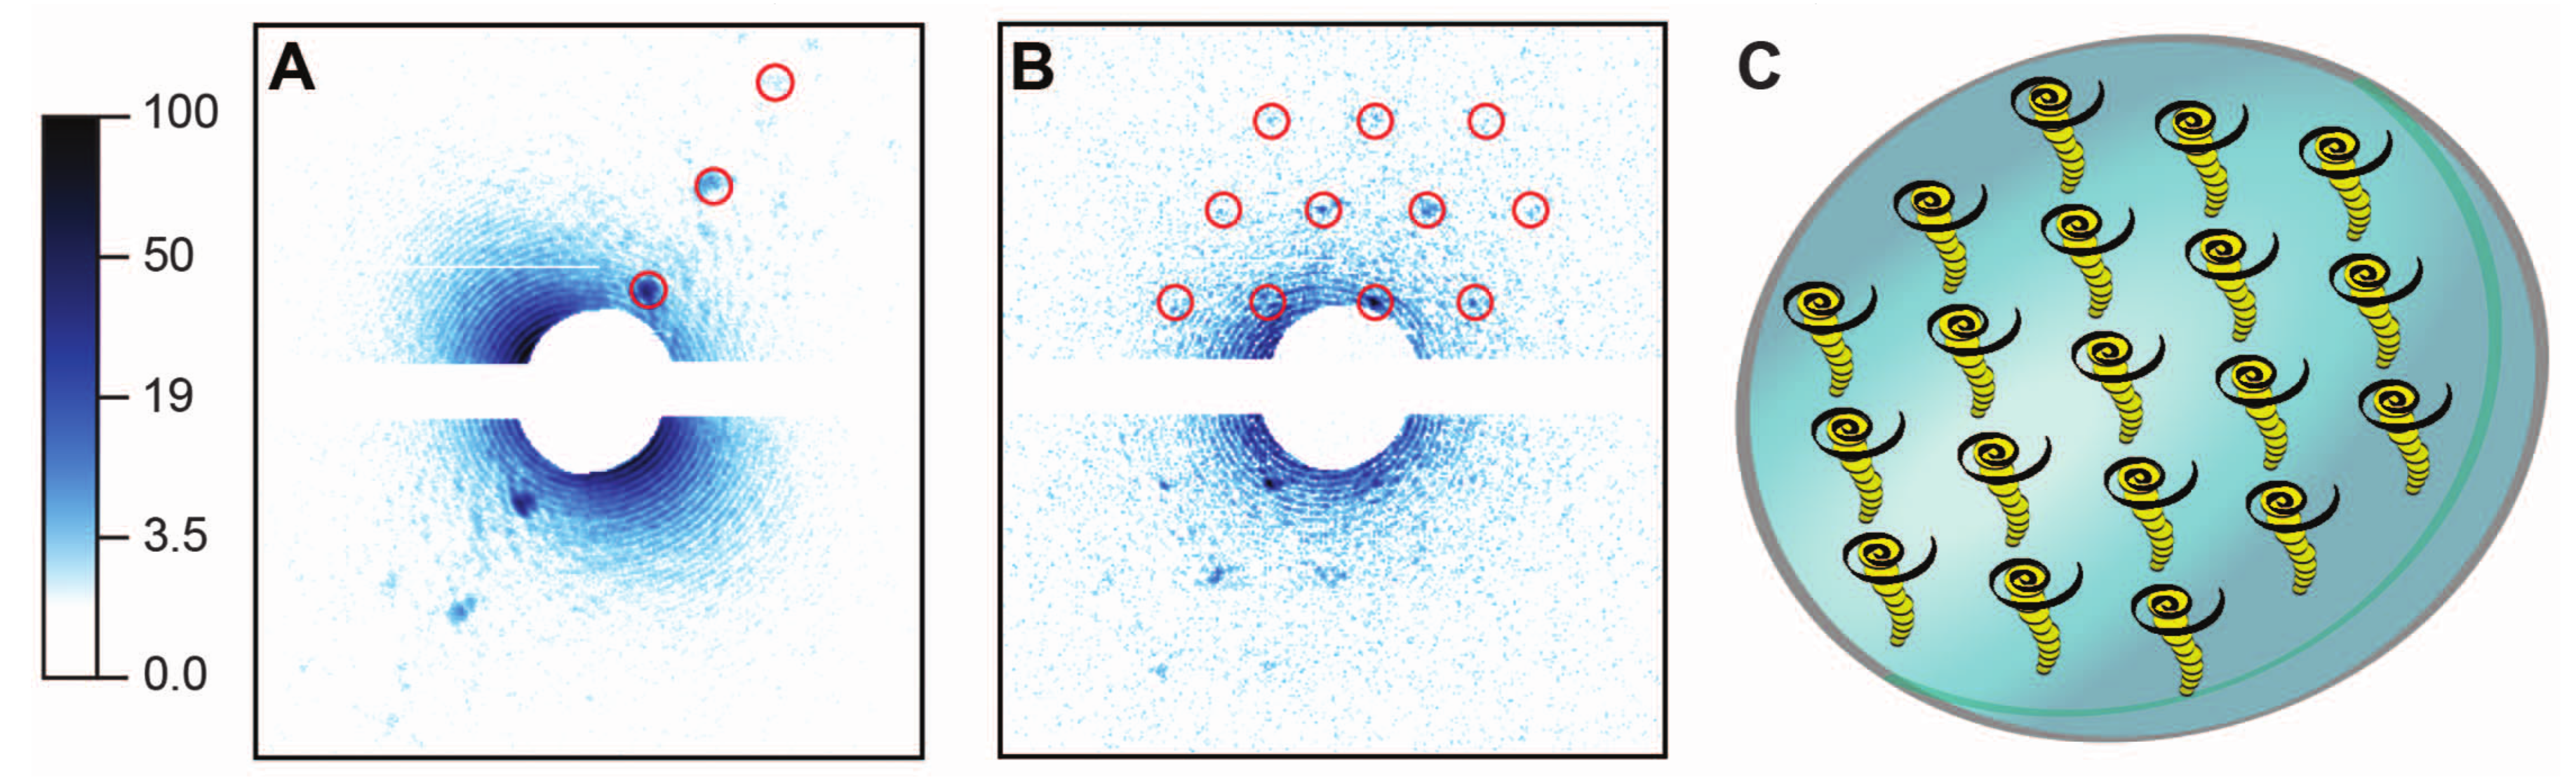
\includegraphics[width=\textwidth]{vortex-array}
			\end{center}
			\caption{He droplets doped with Xe atoms. (A and B) X-ray diffraction images of doped droplets, displayed in a logarithmic intensity scale. (C) Droplet and embedded Xe clusters. Images in (A) and (B) correspond to tilted and parallel alignments of the vortex axes with respect to the incident x-ray beam, respectively.}
			\label{fig:vortex-array}
		\end{figure}
		
		From the theoretical point of view, superfluid helium must be considered as a high dimensional quantum system. Quantum Monte Carlo (QMC) \cite{Kro02} and direct quantum mechanical \cite{deL06,deL10,Agu13} calculations are the most accurate methods, but their computational demand quickly exceeds currently available computer resources when the number of helium atoms increases. Furthermore, QMC cannot describe dynamic evolution of superfluid helium in real time. To address these limitations, approximate methods based on  density functional theory (DFT) formalism have been introduced \cite{Str87a,Str87b,Dal95}. DFT can be applied to much larger systems than QMC and allows for time-dependent formulation. As such, it offers a good compromise between accuracy and computational feasibility. The main drawback of DFT is that the exact energy functional is not known and must therefore be constructed in a semi-empirical manner. Nevertheless, DFT is the only method to date that can successfully reproduce results from a wide range of time-resolved experiments in superfluid helium on the atomic scale.\\
		
	A lot of of work has been done on helium droplets the last, both experimentally and theoretically. From the absorption spectra of alkali metal doped helium droplets, the study of doped mixed $^3$He--$^4$He droplets, electrons in liquid helium, to the investigation of the critical Landau velocity inside small $^4$He droplet. For a comprehensive overview of work done in the last two decades I would like to refer you to some review papers[JLTP.Vol142.Nos.1/2(2006), IRPC.Vol36No4.621-707(2017), IRPC.Vol33No3.301-339(2014)].
	
	\newpage
	\section{Some key concepts}
	I will introduce briefly some key concepts that are used throughout the thesis and that are needed to fully appreciate the discussed material. Also references to more complete and more in-depth treatments will be provided for the interested reader.
		
		\subsection{Bose-Einstein condensation and long-range order}
			The essential concept of Bose-Einstein condensation is the fact that at low temperatures, multiple bosons, unlike fermions, can occupy the same quantum state. In theory there is no upper bound of how many bosons can occupy a single quantum state. It is then said that, with ever decreasing temperature, a macroscopic part of the total number of bosons will ``condense'' into the quantum state with the lowest energy.\\
			
			\begin{align}
				n^{(1)}(\vec{r},\vec{r'}) \vcentcolon= \expectationvalue{\hat{\Psi}^\dagger(\vec{r})\,\hat{\Psi}(\vec{r'})}\label{eq:def-obd-matrix}
			\end{align}
			
			Another important concept in BEC is the idea of long-range order. Once it is accepted that a macroscopic part of the total number of bosons can occupy a single quantum state it can be demonstrated that, while considering a uniform isotropic sytem of $N$ bosons, the one-body density matrix (Eq. \ref{eq:def-obd-matrix}) tends to a constant value when the distance between $\vec{r}$ and $\vec{r}'$ goes to infinity. In the thermodynamic limit where $N,V\rightarrow\infty$ such that $n=N/V$ kept fixed, the one-body density only depends on the modulus of the relative variable $\vec{s}:=\vec{r}-\vec{r}'$ so that we can write it as the Fourier transform of the momentum distribution like so
			\begin{align}
				n^{(1)}(s) = \frac{1}{V}\int \! n^{(1)}\qty(\vec{p})\exp(i\vec{p}\cdot\vec{s}/\hbar)\,\mathrm{d}\vec{p}
			\end{align}
			For a Bose-Einstein condensed system, the momentum distribution at small momenta is not smooth but rather has a form not unlike
			\begin{align}
				n(\vec{p})=N_0\delta(\vec{p})+\tilde{n}(\vec{p})
			\end{align}
			so that in the limit where $s$ goes to infinity
			\begin{align}
				\lim_{s\rightarrow\infty}n^{(1)}(s)=\frac{N_0}{V},
			\end{align}
			where $N_0/V \vcentcolon= n_0\leq 1$ is called the condensate fraction. It is called long-range order since it involves the off-diagonal elements of the one-body density matrix; the elements that are usually associated with the coherences.\\
			
			A set of eigenvalues \{$n_i$\} of the one-body density matrix can be defined through the following eigenvalue equation
			\begin{align}
				\int \! n^{(1)}(\vec{r},\vec{r'})\varphi_i(\vec{r'}) \,\mathrm{d}\vec{r'} = n_i\varphi_i(\vec{r})
			\end{align}
			and its solutions \{$\varphi_i$\} form a natural orthonormal basis set of single boson wave functions $\int\!\varphi_i^*\varphi_j\,\mathrm{d}\vec{r}=\delta_{ij}$, with normalisation condition $\sum_i n_i=N$. This permits writing the on-body density matrix in a useful diagonalised form and recalling that Bose-Einstein condensation occurs when a single particle state $\varphi_i$ is occupied in a macroscopic way, say when $n_{i=0}=N_0$, a number of order $N$, we separate the condensate part from the rest
			\begin{align}
				n^{(1)}(\vec{r},\vec{r'}) = N_0\varphi_0^*(\vec{r})\varphi_0(\vec{r'})+\sum_{i\neq0}n_i\varphi_i^*(\vec{r})\varphi_i(\vec{r'}) \label{eq:obdm-diag}
			\end{align}

		\subsection{Bogolyubov's approximation and the order parameter}
			It is customary, given the importance of the condensate fraction $N_0$ in a BEC, to write, just as the one-body density matrix, the field operator of a $N$-body boson system as the sum of the condensate part and the rest
			\begin{align}
				\hat{\Psi}(\vec{r})=\varphi_0(\vec{r})\hat{a}_0 + \sum_i \varphi_i(\vec{r})\hat{a}_i \label{eq:field-operator}
			\end{align}
			where the $\hat{a}_i$ and $\hat{a}_i^\dagger$ are annihilation and creation operator of a particle in state $\varphi_i$ and obey the usual bosonic commutation relations
			\begin{align}
				\commutator{\hat{a}_i}{\hat{a}_j^\dagger}=\delta_{ij},\quad 	\commutator{\hat{a}_i}{\hat{a}_j}=0=\commutator{\hat{a}_i^\dagger}{\hat{a}_j^\dagger}
			\end{align}
			Using Eq. (\ref{eq:field-operator}) in Eq. (\ref{eq:def-obd-matrix}) and comparing it to Eq. (\ref{eq:obdm-diag}) one finds the expectation value of $\expectationvalue{\hat{a}_j^\dagger\,\hat{a}_i}=\delta_{ij}n_i$. Now, the Bogolyubov approximation consists of replacing the operators $\hat{a}_0$ and $\hat{a}_0^\dagger$ with the $c$-number $\sqrt{N_0}$. This is equivalent to ignoring the non-commutative nature of the operators due to the macroscopic occupation of the state $\varphi_0$ where $N_0=\expectationvalue{\hat{a}_0^\dagger\,\hat{a}_0}\gg 1$. We then rewrite the field operator as the sum of a classical field for the condensed component and quantum field for the non-condensed component
			\begin{align}
				\hat{\Psi}(\vec{r})=\Psi_0(\vec{r})+\delta\hat{\Psi}(\vec{r}),
			\end{align}
			where $\delta\hat{\Psi}(\vec{r})=\sum_{i\neq 0}\varphi_i(\vec{r})\hat{a}_i$ and $\Psi_0(\vec{r})=\sqrt{N_0}\varphi_0(\vec{r})$. At $T=0\unit{K}$ the whole system is condensed and one can ignore $\delta\hat{\Psi}$ altogether; the field operator coincides with the classical field $\Psi_0$ and thus behaves like a classical object.\\
			
			The classical field $\Psi_0$ is called the wave function of the condensate and behaves like an order parameter. It is a complex quantity characterised by a real-valued modulus and phase $S$:
			\begin{align}
				\Psi_0(\vec{r}) = \absolutevalue{\sqrt{N_0}\varphi_0(\vec{r)}}\,\mathrm{e}^{iS(\vec{r})}\label{eq:order-parameter}
			\end{align}
			The modulus determines the number-density of the condensate, while the phase $S$ plays an important role in the coherence and properties of the superfluid. As we will see in Section \ref{sec:rot-vort}, $S$ plays the role of a velocity potential.\\
			
			One way to see why this wave function plays the role of an order parameter is to look at its time dependence. For normal wave functions the time dependence is determined by the eigenvalues $E_i$ of the Hamiltonian of the system
			\begin{align}
				\Psi(\vec{r},t)=\psi(\vec{r})\,\mathrm{e}^{-iE_it/\hbar}
			\end{align}
			But in this case, the time dependence is determined by the chemical potential $\mu=E(N)-E(N-1)\approx \partial E/\partial N$
			\begin{align}
				\Psi_0(\vec{r},t)=\Psi_0(\vec{r})\,\mathrm{e}^{-i\mu t/\hbar}
			\end{align}
			Another aspect of $\Psi_0$ being an order parameter and not a true many-body wave function is that two solutions $\Psi_a$ and $\Psi_b$ are not necessarily orthogonal, i.e. $\int\!\Psi_a^*\Psi_b\unit{d}\vec{r}\neq 0$. However, in dilute gases it is easy to construct a many-body wave function from the order parameter that regains its orthonormality in the thermodynamic limit
			\begin{align}
				\Phi_0(\vec{r}_1,\vec{r}_2,\ldots,\vec{r}_N) = \qty(\frac{1}{\sqrt{N}}\Psi_0(\vec{r}_1))\qty(\frac{1}{\sqrt{N}}\Psi_0(\vec{r}_2))\cdots\qty(\frac{1}{\sqrt{N}}\Psi_0(\vec{r}_N))
			\end{align}
			
		\subsection{Landau's criterion for superfluidity}
		\begin{figure}[t]
			\begin{center}
				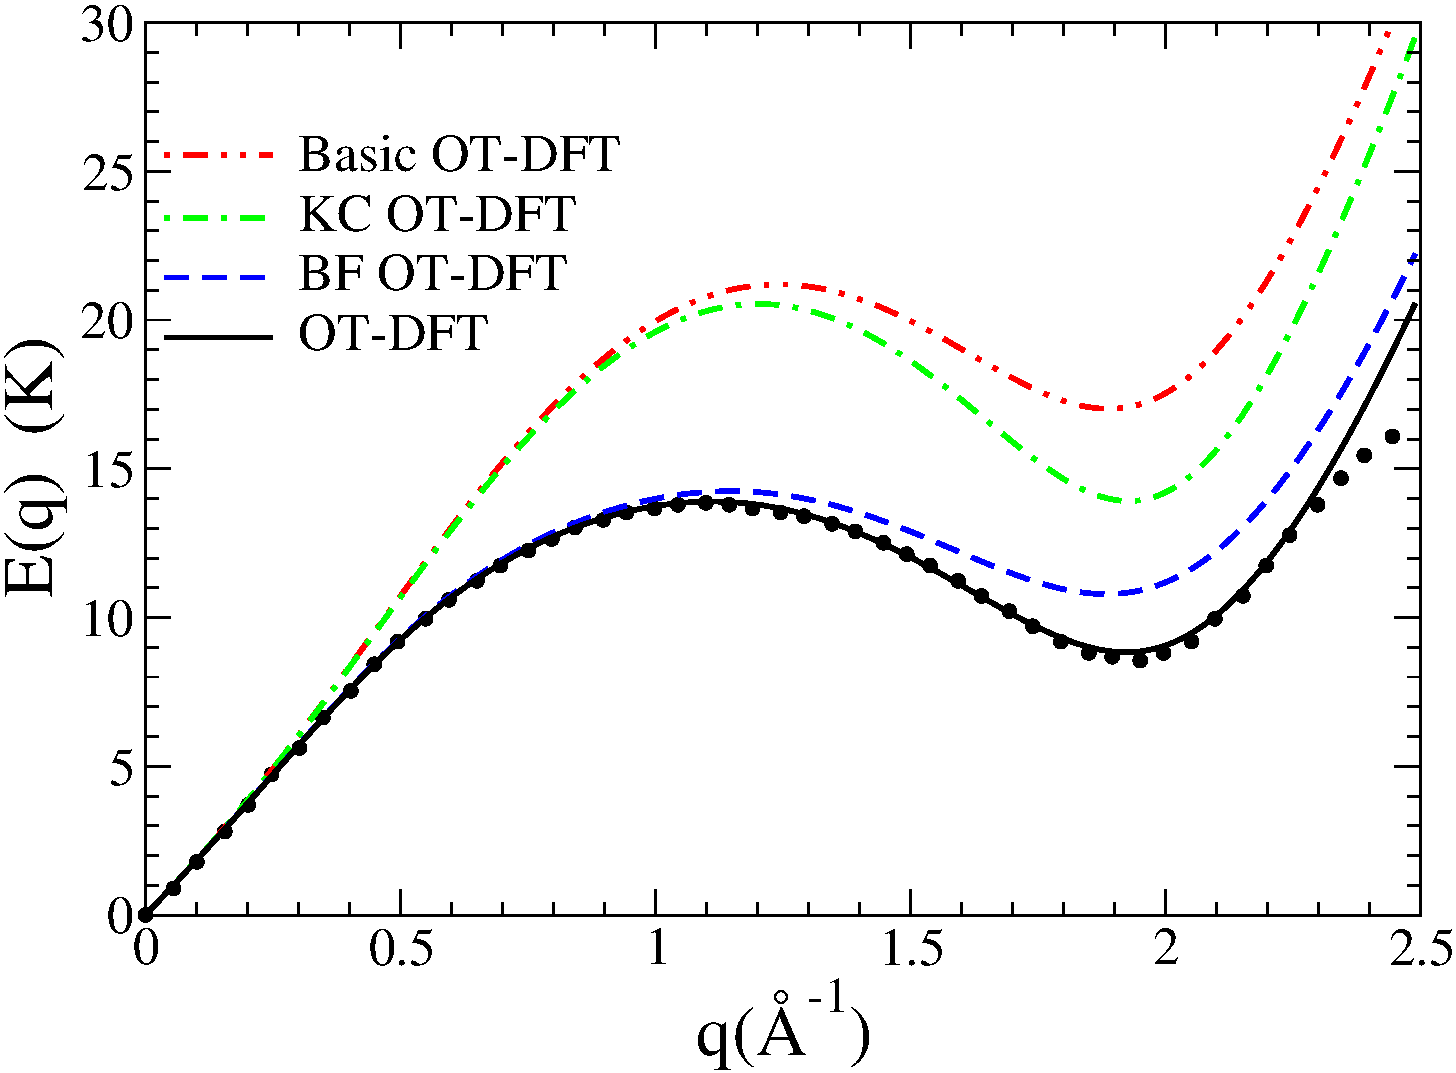
\includegraphics[width=0.9\textwidth]{dispersion-relation}
			\end{center}
			\caption{Dispersion relation for elementary excitations in liquid $^4$He calculated as in  \cite{Mat10a}. `Basic' indicates the OT-DFT without the non-local kinetic energy correlation (KC) nor the back-flow (BF) terms; KC OT-DFT adds  to the basic OT-DFT the KC term; BF OT-DFT adds to the basic OT-DFT the BF term. The dots are the experimental data from \cite{Don81}. The Landau velocity $v_L = E(q)/(\hbar\,q)|_{min}$ obtained for each functional is  60.3 m/s (OT-DFT); 75.1 m/s (BF OT-DFT); 94.4 m/s (KC OT-DFT); 118 m/s (basic OT-DFT); and 57.5 (experiment).}
			\label{fig:dispersion-relation}
		\end{figure}
		
			For a gas or liquid to be able to become superfluid Landau postulated that the energy dispersion relation needs to fulfil certain requirements. Specifically for a fluid to flow  without dissipation, i.e. a super-flow, the velocity field needs to fulfil the following inequality:
			\begin{align}
				v<v_c = \min_{\vec{p}}\frac{\epsilon(\vec{p})}{p}
			\end{align}
			
			For an ideal Bose gas $\epsilon(\vec{p})= \frac{p^2}{2m}$. In this case 
			\begin{align}
				v_c &= \min_{\vec{p}}\frac{\epsilon(\vec{p})}{p} \\
					&= \min_{\vec{p}}\frac{p}{2m} \\
					&= 0
			\end{align}
			Apparently ideal Bose-gases cannot become superfluid.\\
			
			But if we allow for some weak interactions between the bosons the energy dispersion relation becomes
			\begin{align}
				\epsilon(\vec{p})=\sqrt{\frac{gn}{m}p^2+\qty(\frac{p^2}{2m})^2},
			\end{align}
			Bogolyubov's dispersion law for elementary excitations, 1947. And thus
			\begin{align}
				v_c &=\min_{\vec{p}}\sqrt{\frac{gn}{m}+\frac{p^2}{4m^2}} \\
					&= \sqrt{\frac{gn}{m}} \\
					&= c,
			\end{align}
			the speed of sound. Here $g=\frac{4\pi\hbar^2a}{m}$, and $a$ the $s$-wave scattering length. The weakly interacting Bose gases can become superfluid.\\			

			Liquid helium below the $\lambda$-point has a similar energy dispersion relation (see Figure \ref{fig:dispersion-relation}) hence reinforcing the notion that superfluids and BEC's are intimately related. The experimental value of the speed of sound is $\sim\!57.5\unit{m/s}$.
			
		\subsection{Rotation and vorticity in superfluids}\label{sec:rot-vort}
		\begin{figure}[t]
			\begin{center}
				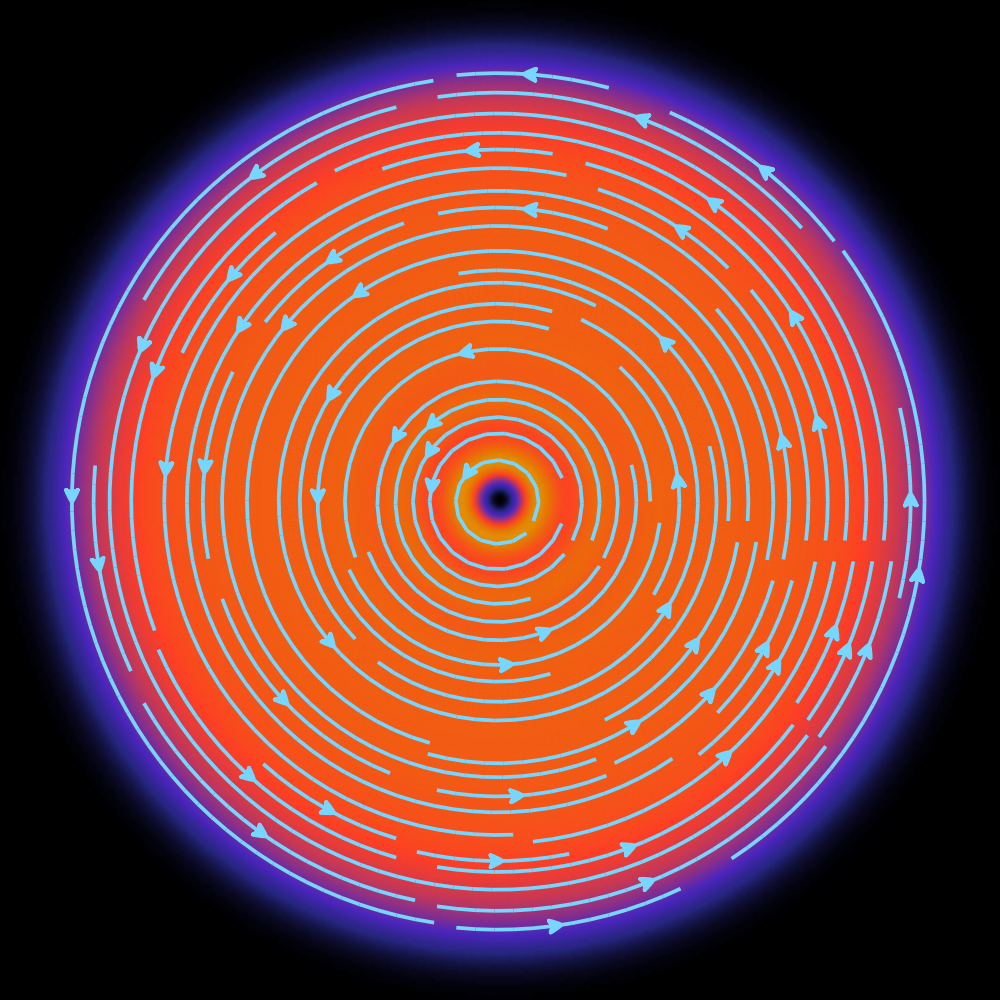
\includegraphics[width=0.75\textwidth]{vortex-xy}
			\end{center}
			\caption{Cross section of a $^4$He droplet through a symmetry plane. The droplet is made of 1000 atoms. Superimposed in cyan are the streamlines of the velocity field $\vec{v}_s$ for $s=1$. They are concentric circles, centred around the vortex core along the $z$-axis. The colour scale encodes for the density $\rho(r)$. The radius of the droplet is about 22\,\AA.}
			\label{fig:vortex-xy}
		\end{figure}
		
			Starting from the EL-equation for the time-evolution of the order parameter it is straightforward to define the current density
			\begin{align}
				\vec{j}(\vec{r},t) \vcentcolon= -\frac{i\hbar}{2m}\qty(\Psi^*\grad{\Psi} - \Psi\grad{\Psi^*})
			\end{align}
			Using a slightly modified expression for the order parameter Eq. (\ref{eq:order-parameter}), identifying the condensate fraction $N_0$ with the superfluids density $\rho$ and making the density and the phase a function of space and time: $\Psi(\vec{r},t) = \sqrt{\rho(\vec{r},t)}\unit{e}^{iS(\vec{r},t)}$ it is straightforward to show that
			\begin{align}
				\vec{j}(\vec{r},t) = \rho(\vec{r},t)\frac{\hbar}{m}\grad{S(\vec{r},t)}
			\end{align} 
			We can then identify the collective velocity $\vec{v}_s$ of the superfluid through the relation
			\begin{align}
				\vec{v}_s(\vec{r},t) = \vec{j}/\rho=\frac{\hbar}{m}\grad{S(\vec{r},t)},
			\end{align}
			and we immediately see that the velocity field of the superfluid is \emph{irrotational}; a typical property of superfluids. Conversely, taking the curl of $\curl{\vec{j}}=\frac{\hbar}{m}\grad{\rho}\times\grad{S}$ we see that this is merely a restatement of the fact that one needs a gas or liquid with a non-uniform density and a non-uniform phase for it to be able to support vortices.\\
			
			Let's consider the prototypical example of a line vortex through the origin along the $z$-axis. Such a vortex solution has the form
			\begin{align}
				\Psi_s(\vec{r}) = \sqrt{\rho(r)}\unit{e}^{is\varphi},
			\end{align}
			in cylinder coordinates with $s$ an integer. This is an eigenfunction of the angular momentum operator $\hat{L}_z$ with eigenvalue
			\begin{align}
				\hat{L}_z \Psi_s(\vec{r}) &= \frac{\hbar}{i}\frac{\partial}{\partial\varphi}\Psi_s(\vec{r}) = \hbar s\Psi_s(\vec{r})
			\end{align}
			and with expectation value
			\begin{align}
				\expval{\hat{L}_z} &= \expval{\hat{L}_z}{\Psi_s} \\
					&= \hbar s \braket{\sqrt{N_0}\varphi_0} \\
					&= N_0\hbar s
			\end{align}
			The angular momentum is quantised and proportional to the number of bosons in the BEC fraction/superfluid. We can calculate the velocity field and the circulation, like so
			\begin{align}
				\vec{v}_s = \frac{\hbar}{m}\grad{S} = \frac{\hbar}{m}\frac{s}{r}\,\vu*{\varphi}
			\end{align}
			The streamlines of $\vec{v}_s$ are concentric circles, centred around the z-axis, lying in the $xy$-plane (see Figure \ref{fig:vortex-xy}). Contrary to rigid rotation fields which increase proportional to the distance from the $z$-axis $r$, the superfluid rotation field decreases proportional to distance from the $z$-axis $1/r$ and is singular in the origin. Calculating the circulation of the velocity field $\vec{v}_s$ along a closed contour including the $z$-axis gives
			\begin{align}
				\oint_{\partial\Sigma}\!\vec{v}_s\cdot\unit{d}\vec{l} &=
				\int\displaylimits_{0}^{2\pi}\!\!\int\displaylimits_{0}^{R}\!\frac{\hbar}{m}\frac{s}{r}\,\vu*{\varphi}\cdot r\unit{d}r\unit{d}\varphi\,\vu*{\varphi} \\
					&= 2\pi s\frac{\hbar}{m}
			\end{align}
			There a two things to note here. Firstly, the circulation around a closed loop that encompasses the $z$-axis is quantised in units of $\hbar/m$ for $s\in\mathbb{N}_{>0}$. Secondly, the value of the circulation of the velocity field does not depend on the chosen contour as long as it includes the location of the vortex. This means that all the vorticity is contained at the location where the velocity field is singular (the ``core'' of the vortex), at $r=0$ along the $z$-axis.\\
			
			Because of the pole in the velocity field, Stokes theorem will lead to the following contradiction
			\begin{align}
				2\pi s\frac{\hbar}{m}=\oint_{\partial\Sigma}\!\vec{v}_s\cdot\unit{d}\vec{l} = \iint_{\Sigma}\!\curl{\vec{v}_s}\cdot\unit{d}\vec{\Sigma} = 0
			\end{align}
			and can therefore not be applied. Formally it is customary to write
			\begin{align}
				\curl{\vec{v}_s} = 2\pi s\frac{\hbar}{m}\delta^{(2)}(\vec{r}_\perp)\,\vu{z},
			\end{align}
			where $\delta^{(2)}$ is 2-dimensional Dirac-delta function and $\vec{r}_\perp$ a vector in a plane perpendicular to the vortex line.\\

	\newpage
	\section{Structure of the thesis}
		The thesis will consist of two parts, since the presented work focusses on two distinct areas of interest with no mutual overlap. Each part will have its own short introduction to motivate the performed research and put in a broader context. The final chapter contains a more general discussion about the presented material and will conclude with some work in progress and future prospects.

		\subsection{Part I: Excited state dynamics}
			In this part of the thesis the real-time dynamics of a single electronically excited rubidium (Rb) atom, residing in the surface dimple of a helium nano-droplet will be presented. The atom will be excited from its ground state 5s$^2\Sigma_{1/2}$ to the 5p$^2\{\Sigma,\Pi\}$ and 6p$^2\{\Sigma,\Pi\}$ manifold. This will be a combined experimental and theoretical study. The results are presented in two published articles:\\
		
			\emph{Imaging Excited-State Dynamics of Doped He Nanodroplets in Real-Time} will focus on imaging and characterising the dynamics using femtosecond spectroscopy and  time-dependent density functional theory.\\
		
			\emph{Desorption dynamics of RbHe-exciplexes off He nanodroplets induced by spin relaxation} is a combined experimental and theoretical investigation of the formation of free RbHe-exciplex molecules from laser-excited Rb-doped He nanodroplets through the mechanism of electronic spin relaxation. The role of relaxation of internal degrees of freedom of the RbHe exciplex in the desorption process has not been explicitly addressed.

		\subsection{Part II: Collisions and capture by quantised vortices}
			The second part investigates the real-time capture process of single xenon and argon atoms in their ground state by $^4$He$_{1000}$ droplets. Specifically it will address the interaction between a captured xenon or argon atom and a single quantised vortex line in the interior of the droplet. It will contain only theoretical investigations. The results will also be presented in two published works:\\
		
			\emph{Head-on Collisions of Xe Atoms Against Superfluid $^4\!$He Nanodroplets} studies the kinematics of head-on collisions between a xenon atom and a helium droplet. This scenario is then compared to a previous study of the same process with caesium to get a clear picture of the differences in dynamic behaviour between heliophilic and heliophobic species in said process. It also investigates different velocity regimes.\\
		
			\emph{Capture of Xe and Ar atoms by quantized vortices in $^4\!$He nanodroplets} addresses the capture of xenon and argon atoms at different velocity regimes and impact factors to determine the effective cross section for capture. This investigation then repeated with a dropet hosting one quantised line vortex. Also some preliminary results are presented for a larger droplet hosting an array of 6 line vortices, lined with argon atoms.

		\newpage
		\section{The method of Density Functional Theory}
		
			The starting point is the Hohenberg-Kohn (HK) theorem \cite{Hoh64}, which states that the total energy $E$ of a many-body quantum system at $T=0$ is a functional of the one-particle density
			\begin{align}
				E[\rho] = {\cal T}[\rho] +\int\!{\cal E}[\rho]\label{eq1}\diff{\vec{r}}
			\end{align}
			with $\rho ({\mathbf r})= \langle\Phi |\hat\rho(\vec{r})|\Phi \rangle \vcentcolon= \langle\Phi |\sum _{i=1}^{N} \delta ({\mathbf r}-{\mathbf r}_i)|\Phi \rangle$ and $\Phi$ the many-body wave function.
			Kohn and Sham reformulated this such that we can write this expression as 
			\begin{equation}
				E[\rho] = T[\rho] + \int\!{\cal E}_c[\rho]\diff{\vec{r}} \label{eq2}
			\end{equation}
			where this time
			\begin{equation}
				T= -\frac{\hbar^2}{2m_4} \sum_i \int\! \phi _i^\ast ({\mathbf r})\nabla^2  \phi _i ({\mathbf r})\diff{\vec{r}} \label{eq3}
			\end{equation}
			is the kinetic energy of a system of $N$ non-interacting particles and 
			As before def $\Psi(\textbf{r}) = \sqrt{N_4} \phi_0(\textbf{r})$. Then
			\begin{align}
				T[\rho] =
				-\frac{\hbar^2}{2m_4} N_4 \langle \phi_0 | \nabla^2 \phi_0\rangle = \frac{\hbar^2}{2m_4} \int d {\mathbf r} |\nabla \Psi|^2 \label{eq5}
			\end{align}
			\begin{align}
				\imath \hbar\frac{\partial}{\partial t} \Psi({\mathbf r},t) = \left\{-\frac{\hbar^2}{2m_4}\nabla^2 + \frac{\delta{\cal E}_{c}}{\delta\rho}\right\}\Psi(\textbf{r},t)  \equiv {\cal H}\left[\rho\right] \,\Psi(\textbf{r},t) 
				\label{eq6}
			\end{align}
Def: $\Psi(\vec{r},t) = \Psi_0(\vec{r})\unit{e}^{-i\mu t/\hbar}=\absolutevalue{\sqrt{N_0}\varphi_0(\vec{r)}}\unit{e}^{i\qty[S(\vec{r})-\mu t/\hbar]}$
			\begin{align}
			\left\{-\frac{\hbar^2}{2m_4} \nabla^2 + \frac{\delta {\cal E}_{c}}{\delta \rho}\right\}\Psi_0(\textbf{r}) = \mu \Psi_0(\textbf{r})
			\label{eq7}
			\end{align}
			
			\begin{eqnarray}
			{\cal E}_c[\rho ,\mathbf{v}] &=&  
			\frac{1}{2} \int {\rm d}{\bf r'} \rho({\bf r}) V_{LJ}(|{\bf r}-{\bf r'}|) \rho({\bf r'}) 
			\nonumber \\
			&& + \frac{1}{2} c_2\, \rho({\bf r}) \left[{\bar \rho}({\bf r}) \right]^2 
			+ \frac{1}{3} c_3 \, \rho({\bf r}) \left[ {\bar \rho}({\bf r}) \right]^3 
			\nonumber \\
			&&- \frac{\hbar^2}{4m_4} \alpha_s \int {\rm d}{\bf r'} F(|{\bf r}-{\bf r'}|) 
			\left[ 1- \frac{{\tilde \rho}({\bf r})}{\rho_{0s}} \right]
			\nabla \rho({\bf r}) \cdot \nabla' \rho({\bf r'})
			\left[ 1- \frac{{\tilde \rho}({\bf r'})}{\rho_{0s}} \right] 
			\nonumber
			\\
			&& - \frac{m_4}{4} \int d\mathbf{r}' \,V_J(| \mathbf{r} - \mathbf{r}'|)\, \rho(\mathbf{r}) \, \rho(\mathbf{r}')\,  [\mathbf{v}(\mathbf{r}) - \mathbf{v}(\mathbf{r}')]^2
			\label{eq8}
			\end{eqnarray}		
			
			\begin{table}[t]
			Model parameters for the OT-DFT and solid functionals.
			\vspace{50pt}
			{\begin{tabular}{@{}lccccc}
			\hline
			\hline
			$\epsilon_{LJ}$  (K)    & $\sigma$ (\AA)& $h$ (\AA) & $c_2$ (K \AA$^6$)  & $c_3$ (K \AA$^9$) & $\alpha_s$ (\AA$^3$) \\
			 10.22   & 2.556 & 2.190323 & $-$2.41186 $\times 10^4$ & 1.85850 $\times 10^6$ & 54.31 \\
			\hline
			 $\rho_{0s}$ (\AA$^{-3}$)& $l$ (\AA)&$C$ (Hartree) &$\beta$ (\AA$^3$) & $\rho_m$ (\AA$^{-3}$) & $\gamma_{11}$ \\  
			  0.04& 1. & 0.1 &40.   & 0.37 & $-$19.7544 \\
			  \hline
			  $\gamma_{12}$ (\AA$^{-2}$)& $\alpha_1$  (\AA$^{-2}$) & $\gamma_{21}$  & $\gamma_{22}$ (\AA$^{-2}$) & $\alpha_2$ (\AA$^{-2}$) &      \\  
			   12.5616 &1.023 &  $-$0.2395 & 0.0312 & 0.14912  & \\
			\hline
			\hline
			\end{tabular}}
			\label{table1}
			\end{table}
			
			\begin{align}
				V_{LJ}(r) = \begin{cases}
				\epsilon_{LJ} \left[ \left(\frac{\sigma}{r} \right)^{12} - \left(\frac{\sigma}{r} \right)^{6} \right] & {\rm if} \quad r > h \\
				0 & {\rm otherwise}
				\end{cases}\label{eq9}
			\end{align}
			
			\begin{equation}
			V_J(r) = (\gamma_{11} +\gamma_{12} \, r^2) e^{-\alpha_1 r^2}+(\gamma_{21} +\gamma_{22} \, r^2) e^{-\alpha_2 r^2}
			\label{eq15}
			\end{equation}
			
			\begin{equation}
{\bar \rho}({\bf r}) = \int {\rm d}{\bf r'} \rho({\bf r'}) w(|{\bf r}-{\bf r'}|)
\label{eq11}
\end{equation}
%
where
%
\begin{eqnarray}
w(r) &=& \frac{3}{4 \pi h^3} \quad {\rm if} \quad r <h \nonumber \\
&=& 0 \quad {\rm otherwise.} 
\label{eq12}
\end{eqnarray} 
%
and 
%
\begin{equation}
{\tilde \rho}({\bf r}) = \int {\rm d}{\bf r'} \rho({\bf r'}) F(|{\bf r}-{\bf r'}|)
\label{eq13}
\end{equation}
%
where $F(r)$ is a Gaussian kernel
%
\begin{equation}
F(r)= \frac{1}{\pi^{3/2}l^3} {\rm e}^{-r^2/l^2}
\label{eq14}
\end{equation}

			\subsubsection{Static calculations}
				\begin{equation}
E[\rho] \rightarrow E[\rho] +  \int d {\mathbf r} \rho({\mathbf r}) V_X(|{\mathbf r} - {\mathbf r}_I|)  
\label{eq20}
\end{equation}

				\begin{equation}
\left\{-\frac{\hbar^2}{2m_4} \nabla^2 + \frac{\delta {\cal E}_c}{\delta \rho}  + V_X(|{\mathbf r} - {\mathbf r}_I|) \right\}\Psi({\mathbf r})  
= \mu \Psi({\mathbf r})
\label{eq21}
\end{equation}

			\begin{equation}
\Psi(\mathbf{r}) = \frac{\rho_0^{1/2}(\mathbf{r})}{\sqrt{x^2 + y^2}} \, (x + \imath y)
\label{eq28}
\end{equation}

\begin{equation}
[{\cal H}-\omega \hat{L}_z] \,  \Psi  (\mathbf{r})  =  \,\mu \,
\Psi (\mathbf{r}) \;,
\label{eq31}
\end{equation}

\begin{equation}
\Psi(\mathbf{r})=\rho_0^{1/2}(\mathbf{r})\, \prod _{j=1}^{n_v} \left[ {(x-x_j)+\imath (y-y_j) \over \sqrt{(x-x_j)^2+(y-y_j)^2}}  \right] 
\label{eq32}
\end{equation}

			\subsubsection{Dynamic calculations}

\begin{equation}
E[\rho] \rightarrow E[\rho] + \frac{p^2_I}{2 m_I} + \int d \mathbf{r} \, \rho(\mathbf{r}) \,  V_{X^*}(|\mathbf{r}- \mathbf{r}_I|) 
 \label{eq33}
\end{equation}

\begin{eqnarray}
i\hbar\frac{\partial}{\partial t} \Psi
&=&
\left[
  -\frac{\hbar^2}{2m_4} \nabla^2 +
  \frac{\delta {\cal E}_c}{\delta \rho}
  +
  V_{X^*}(|\mathbf{r}- \mathbf{r}_I|)
\right]
\Psi
\nonumber
\\
m_I \ddot{\mathbf{r}}_I
&=&
- \nabla_{\mathbf{r}_I}
\left[  \int d \mathbf{r} \,\rho(\mathbf{r}) V_{X^*}(|\mathbf{r}- \mathbf{r}_I|)  \right]  =
-  \int d \mathbf{r} \, V_{X^*}(|\mathbf{r}- \mathbf{r}_I|)  \, \nabla \rho(\mathbf{r})  
 \;
\label{eq34}
\end{eqnarray}

\begin{equation}
U(r_n)= 
V_{\Pi}(r_n)\mathbf{I}+\{V_{\Sigma}(r_n)-V_{\Pi}(r_n)\}|p_{zn}\rangle\langle p_{zn} |  
\label{eq37}
\end{equation}
%
where $r_n$ is the interatomic distance and $V_\Pi(r)$ and $V_\Sigma(r)$ are the $\Pi$ and $\Sigma$ impurity-He pair potentials in the absence of spin-orbit coupling.

For a system consisting of $N_4$ helium atoms and an excited p-state impurity, the total potential energy is constructed using the DIM model \cite{Ell63}
%
\begin{equation}
U=\sum_{n=1}^{N_4}\left\{V_\Pi(r_n)\mathbf{I}+[V_\Sigma(r_n)-
V_\Pi(r_n)] R_n |p_z\rangle\langle p_z | R^{-1}_n\right\}  
\label{eq38}
\end{equation}
%
where $R_n$ is a rotation matrix which transforms the common laboratory frame to the diatomic frame corresponding to the $n^{\rm th}$ He atom. 
In cartesian coordinates
%
\begin{equation}
\langle p_i|  R_n |p_z\rangle\langle p_z| R^{-1}_n |p_j\rangle = \frac{r_{in}~r_{jn}}{r_n^2}
\label{eq39}
\end{equation}
%
where $r_{1n}\equiv x_n$, $r_{2n} \equiv y_n$, $r_{3n} \equiv z_n$, and $r_n^2=x_n^2+y_n^2+z_n^2$ for the $n^{\rm th}$ He atom. 
The matrix elements of the DIM Hamiltonian are then
%
\begin{equation}
\langle p_i | U | p_j \rangle\equiv U_{ij}=
\sum_{n=1}^{N_4}\left\{V_\Pi(r_n)\delta_{ij}+
[V_\Sigma(r_n)-V_\Pi(r_n)]\frac{r_{in}~r_{jn}}{r_n^2}\right\}  
\label{eq40}
\end{equation}
%
Since DFT provides a continuous distribution, the discrete sum over helium atoms is replaced by integration over the density 
($\sum_n\rightarrow\int\mathrm{d}^3\mathbf{r''}\rho(\mathbf{r''})$),
which gives
%
\begin{equation}
U_{ij}(\mathbf{r})= \int\mathrm{d}^3\mathbf{r'}\rho(\mathbf{r'}+\mathbf{r})
\left\{V_\Pi(r')\delta_{ij}+[V_\Sigma(r')-V_\Pi(r')]\frac{r'_i~r'_j}{r'^2}\right\} 
\label{eq41}
\end{equation}
%
The eigenvalues $V^{\mathrm{ex}}_m(\mathbf{r})$ of this real symmetric matrix define the potential energy curves (PEC) as a function of the distance between the surrounding helium and the impurity.

The above model assumes that spin-orbit (SO) coupling is negligible. 
However, when it becomes comparable to the helium induced splitting of the p-orbitals, it must be included in the calculation. 
The total Hamiltonian is then given by $U_T = U+U_{SO}$ where $U_{SO}$ is the SO hamiltonian matrix, usually approximated by that of the free atom \cite{Jak97}.
The previously mentioned minimal DIM basis set can be extended to include the electron spin: $s = \uparrow (m_s = $ $^1\!/_2)$, $s= \downarrow (m_s= -^1\!/_2)$, i.e. 
$|i,s \rangle \equiv |p_x, \uparrow \rangle, |p_x, \downarrow \rangle, |p_y, \uparrow \rangle, |p_y, \downarrow \rangle, |p_z, \uparrow \rangle, |p_z, \downarrow \rangle$.

Kramers' theorem states that the two-fold degeneracy of the levels originating from total half-integer spin cannot be broken by electrostatic interactions \cite{Nak01}. 
Thus, all the electronic eigenstates of $U_T$ are doubly degenerate. 
Diagonalization of $U_T$ yields three doubly degenerate PEC between the impurity and surrounding helium. 
This method has also been extended to impurities in D electronic states \cite{Lea16,Mel14}.

The DIM wave function of the impurity, $|\lambda\rangle$, is determined by a six-dimensional state vector
%
\begin{equation}
|\lambda \rangle = \sum_{\mathop{i=x,y,z}\limits_{s=-1/2,1/2}} \lambda_{is} |i,s \rangle \;\; .
\label{eq42}
\end{equation}
%
The complete set of variables required to describe the
system consists of the complex valued effective wave function for helium $\Psi(\mathbf{r}, t)$ with
$\rho(\mathbf{r}, t) = |\Psi(\mathbf{r}, t)|^2$, the impurity position $\mathbf{r}_I(t)$, and the 6-dimensional complex vector to determine 
its electronic wave function $|\lambda(t)\rangle$. The total energy of the impurity-$^4$He$_N$ complex after excitation to the $^2$P manifold is
%
\begin{equation}
E[\Psi, \mathbf{r}_I, \lambda] =
\int d \mathbf{r} \,
\frac{\hbar^2}{2m}|\nabla \Psi|^2
+
\frac{p^2_I}{2 m_I}
+
\int d \mathbf{r} \,
{\cal E}_c[\rho]
+
\langle \lambda | V_{SO} |\lambda\rangle
+ \int d \mathbf{r} \, \rho(\mathbf{r}) \,
 V_\lambda (\mathbf{r}- \mathbf{r}_I ) 
 %\; .
 \label{eq43}
\end{equation}
%
where $V_{SO}$ is the spin-orbit coupling operator and $V_\lambda$ is defined as
%
\begin{equation}
V_\lambda(\mathbf{r}) \equiv \langle \lambda | {\mathcal V}(\mathbf{r}) | \lambda\rangle = \sum_{ijss'}\lambda^*_{is}{\mathcal V}^{ijss'}(\mathbf{r})\lambda_{js'} 
\label{eq44}
\end{equation}
%
with the components of the six-dimensional matrix ${\mathcal V}$ given by
%
\begin{equation}
{\mathcal V}^{ijss'}(\mathbf{r}) =\left[ V_\Pi(r)\delta_{ij} +
\left(V_\Sigma(r)-V_\Pi(r)\right)\frac{r_i r_j}{r^2} \right]\delta_{ss'}
\label{eq45}
\end{equation}

The time evolution of the system is obtained by minimizing the action
%
\begin{equation}
{\cal A}[\Psi, \mathbf{r}_I, \lambda] =
\int dt \left\{ E[\Psi, \mathbf{r}_I, \lambda]  -  i \hbar \int d \mathbf{r} \,
\Psi^*(\mathbf{r}) \frac{\partial}{\partial t} \Psi(\mathbf{r})  - i \hbar 
\langle \lambda | \frac{\partial}{\partial t} | \lambda \rangle - \frac{1}{2} m_I \dot{\mathbf{r}}^2_I \right\} \;
\label{eq46}
\end{equation}
%
Variation of $\cal A$ with respect to $\Psi^*$,  $\langle\lambda|$  and $\mathbf{r}_I$ yields
%
\begin{eqnarray}
&&i\hbar\frac{\partial}{\partial t} \Psi =
\left[
  -\frac{\hbar^2}{2m}\nabla^2 +
  \frac{\delta {\cal E}_c}{\delta \rho(\mathbf{r})}
  +
  V_\lambda(\mathbf{r}- \mathbf{r}_I)
\right]
\Psi
\nonumber
\\
&&i\hbar\frac{\partial}{\partial t} | \lambda \rangle  =
{\cal H} \; |\lambda\rangle
\nonumber
\\
&&m_I\ddot{\mathbf{r}}_I
=
- \nabla_{\mathbf{r}_I}
\left[
  \int d \mathbf{r} \rho(\mathbf{r})
  V_\lambda(\mathbf{r}- \mathbf{r}_I)
  \right] =  -   \int d \mathbf{r} \,  V_\lambda(\mathbf{r}- \mathbf{r}_I)  \nabla \rho(\mathbf{r})
\label{eq47}
\end{eqnarray}
%
where the explicit time dependence of the variables is omitted for clarity.
The second line of Eq. (\ref{eq47}) is a $6\times 6$ matrix equation with the matrix elements given by
%
\begin{equation}
H^{ijss'} = \int d \mathbf{r} \, \rho(\mathbf{r})
 {\mathcal V}^{ijss'} (\mathbf{r}- \mathbf{r}_I)
 + V^{ijss'}_{SO}
 \label{eq48}
\end{equation}
			


%		Introduce superfluids and their properties
%		* Frictionless capillary flow (no viscosity)
%		* Creeping up the walls seemingly defying gravity
%		* capillary fountain
%		* second sound: heat propagating in waves with a constant speed of "second sound" instead of diffusion
%		* Fluid is irrotational
%		* Vorticity is quantised
	 

%%		E, 1908, July 10:		Kamerlingh Onnes, Liquefaction of helium-4,\\
%%		E, 1932, July:			John C. McLennan, Observed liquid helium stops boiling
%below 2.2 K. \\
%%		E, 1932:				W.H. Keesom, A.P. Keesom, observed a singularity in the specific
%heat at T=2.2 K and called it the lambda-temperature, because of the shape of
%the temperature dependence of the specific heat resembling the greek letter
%lambda.\\
%%		E, 1935, February 16:	E.F. Burton, measured sharply decreasing viscosity
%below 2.2 K\\
%%		T, 1935, August 16:		F. London, found that the magnitude of the zero-point
%energy of helium-4 is comparable to the Van der Waals interaction. This
%explains why helium doesn't freeze at T=0 at normal atmospheric pressure.\\
%%		E, 1936, May:			W.H. Keesom, A.P. Keesom, Observed abnormally thermal
%conductance, calling it 'supra-heat-conducting'\\
%%		E, 1937, July 10:		J.F. Allen,R. Peierls, M. Zaki Uddin, also observed
%abnormally high heat conductance. This was the reason for the liquid not
%boiling below 2.2 K\\
%%		E, 1937, December 3:	Kapitza, observed that below lambda-point viscosity of
%helium II is roughly 1500 smaller than helium I at normal pressure. In analogy
%with superconductors he concluded that helium below lambda enters a special
%state which he called superfluid.	This was the first mention of the word
%superfluid.\\
%%		E, 1937, December 22:	Allen and Misener (1938) discovered that helium-ii is
%not just a liquid with a very low viscosity, but that its hydrodynamics
%required a completely new interpretation.\\
%%		E, 1938, 05 February: 	J.F. Allen, discovery of fountain effect\\
%%		T, 1938, April 9:		F. London, connects behaviour of helium-II to BEC (ideal
%BE-gas). calculated Tc=3.09 K and Cv(t) for ideal BE-gas and they were very
%close to helium-II. He concluded that it was difficult not to imagine a
%connection to BEC\\
%%		T, 1938, May 21:		L. Tisza, birth of the 2-fluid model\\
%
%					which leads to 
%
%	Explanation of superfluidity by 
%		* Fritz London (April 1938, London, F., Nature, 141, 643 (1938))
%l-transition in liquid helium is analogous to Bose-Einstein condensation
%%		* Laszlo Tisza (May 1938, L. Tisza, Nature, 141, 913 (1938)) extended
%London's proposal by invoking a two-fluid model for helium II, which could
%qualitatively explain the observed transport phenomena, including the fountain
%effect.
%%		* Lev Landau (1941) if the spectrum of elementary excitations satisfies
%suitable criteria, the flow of of the fluid cannot dissipate energy. Postulated
%"phonons" and "rotons" and the famous Landau criterion for superfluidity
%%		* Nikolay Nikolayevich Bogolyubov (Oct. 12, 1946. Publ. 1947): Derivation of
%the elementary excitation spectrum from a molecular theory, making no
%assumptions about the structure of the energy spectrum.


%	\section{Random stuff about BEC}
%	Most general (time-independent) many-body Hamiltonian
%	\begin{align}
%		H(\vec{r}_1,\ldots,\vec{r}_N, \vec{p}_1,\ldots,\vec{p}_N) =
%\sum_{i=1}^N
%\qty(-\frac{\hbar^2}{2m_i}\nabla_{\vec{r}_i}^2)+V(\vec{r}_i,\ldots,\vec{r}_N)
%	\end{align}
%	And accompanying Schrödinger equation to solve
%	\begin{align}
%		i\hbar\frac{\partial}{\partial t}\Psi(\vec{r}_1,\ldots,\vec{r}_N,t) =
%\qty[\sum_{i=1}^N
%\qty(-\frac{\hbar^2}{2m_i}\nabla_{\vec{r}_i}^2)+V(\vec{r}_i,\ldots,\vec{r}_N)
%]\Psi(\vec{r}_1,\ldots,\vec{r}_N,t)
%	\end{align}
%For a 2-body system and a potential that only depends on the relative
%coordinate $\vec{r}_1-\vec{r}_2$ the Hamiltonian reduces reduces to
%	\begin{align}
%		H(\vec{r}_1,\vec{r}_2) =
%-\qty(\frac{\hbar^2}{2m_1}\nabla_{\vec{r}_1}^2+\frac{\hbar^2}{2m_2}\nabla_{\vec
%{r}_2}^2)+V(\vec{r}_1-\vec{r}_2)
%	\end{align}
%By either introducing the relative coordinate $\vec{r}$ and the center-of-mass
%(CM) coordinate $\vec{R}$, or the relative momentum
%$\vec{p}$ and the total momentum $\vec{P}$, we can consider the motion of the
%CM itself ($\vec{R}$) and the motion relative to the CM
%	($\vec{r}$):
%	\begin{align}
%		H(\vec{R},\vec{r}) =
%-\qty(\frac{\hbar^2}{2M}\nabla_{\vec{R}}^2+\frac{\hbar^2}{2\mu}\nabla_{\vec{r}}
%^2)+V(\vec{r}),
%	\end{align}
%with $M=m_1+m_2$ and $\mu=\frac{m_1m_2}{m_1+m_2}$ (reduced mass of the system).
%	Schrödinger equation to solve
%	\begin{align}
%i\hbar\frac{\partial}{\partial t}\Psi(\vec{R},\vec{r},t) &=
%H(\vec{R},\vec{r})\Psi(\vec{R},\vec{r},t) \\
%&=
%\qty[-\qty(\frac{\hbar^2}{2M}\nabla_{\vec{R}}^2+\frac{\hbar^2}{2\mu}\nabla_
%{\vec{r}}^2)+V(\vec{r})]
%		\Psi(\vec{R},\vec{r},t) \label{eq:2b-se}
%	\end{align}
%	Assuming a separable solution and the given time-independence of the potential
%	\begin{align}
%\Psi(\vec{R},\vec{r},t) =
%\Phi(\vec{R})\psi(\vec{r})\mathrm{e}^{-i(E_{CM}+E)t/\hbar}
%	\end{align}
%and the 2-body Schrödinger equation (\ref{eq:2b-se}) separates into two
%mutually time-independent ODEs
%	\begin{align}
%-\frac{\hbar^2}{2M}\nabla_{\vec{R}}^2\Phi(\vec{R}) &= E_{CM}\Phi(\vec{R})
%\label{eq:se-fp}\\
%\qty[-\frac{\hbar^2}{2\mu}\nabla_{\vec{r}}^2 + V(\vec{r})]\psi(\vec{r}) &=
%E\psi(\vec{r}). \label{eq:se-muv}
%	\end{align}
%ODE (\ref{eq:se-fp}) describes the center of mass motion for a free particle
%with mass $M$ and energy
%$E_{CM}$. In one dimension the time-\emph{dependent normalizable} solution for
%such a particle,
%initially localized between $-a$ and $a$ is an integral over plane waves over
%all frequencies
%	\begin{align}
%\Phi(X,t) =
%\frac{1}{\pi}\sqrt{\frac{a}{2}}\int_{-\infty}^{+\infty}\!\mathrm{sinc}(ka)\,
%		\exp[i\qty(kX-\frac{\hbar k^2}{2M}t)]\,\mathrm{d}k.
%	\end{align}
%ODE (\ref{eq:se-muv}) describes the motion relative to the CM of a particle of
%reduced mass $\mu$ in a potential $V(\vec{r})$.
%	For hydrogen this is the Coulomb potential. Explicitly
%	\begin{align}
%\qty[-\frac{\hbar^2}{2\mu}\nabla_{\vec{r}}^2 -
%\frac{e^2}{(4\pi\varepsilon_0)r}]\psi(\vec{r}) &= E\psi(\vec{r}),
%	\end{align}
%where it is customary to switch to spherical polar coordinates and separate the
%solutions again
%	\begin{align}
%\psi(\vec{r}) \rightarrow \psi_{E,l,m}(r,\theta,\phi) =
%R_{E,l}(r)Y_{ml}(\theta,\phi),
%	\end{align}
%where $R_{E,l}$ is the radial wave function, fully determined by the energy $E$
%and the orbital angular momentum quantum
%number $l$ and $Y_{ml}$ are the spherical harmonics, fully determined by $l$
%and the magnetic quantum number $m$.
%	
%	\section{Helium-4, a 3-body system with 2 electrons}
%The unperturbed (omit electron-electron repulsion) ground state (as obtained by
%the `single particle model')
%	\begin{align}
%\psi_0^{(0)}(r_1,r_2) &= \psi_{1\mathrm{s}(r_1)}\psi_{1\mathrm{s}(r_2)} \otimes
%		\frac{1}{\sqrt{2}}\qty(\ket{\uparrow\downarrow}-\ket{\downarrow\uparrow}) \\ 
%&= \frac{8}{\pi}\exp[-2(r_1+r_2)] \otimes
%\frac{1}{\sqrt{2}}\qty(\ket{\uparrow\downarrow}-\ket{\downarrow\uparrow})
%	\end{align}
%Or in the `central field approximation' with effective nuclear charge
%$Z_e=1.70$
%	\begin{align}
%\psi_0(r_1,r_2) =
%\frac{4.913}{\pi}\exp[-1.70(r_1+r_2)]\otimes\frac{1}{\sqrt{2}}\qty(\ket
%{\uparrow\downarrow}-\ket{\downarrow\uparrow})
%	\end{align}

\end{document}